\documentclass[12pt]{article}

\usepackage{amsthm}
\usepackage{amsmath}
\usepackage{amsfonts}
\usepackage{mathrsfs}
\usepackage{array}
\usepackage{amssymb}
\usepackage{units}
\usepackage{graphicx}
\usepackage{tikz-cd}
\usepackage{nicefrac}
\usepackage{hyperref}
\usepackage{bbm}
\usepackage{color}
\usepackage{tensor}
\usepackage{tipa}
\usepackage{bussproofs}
\usepackage{ stmaryrd }
\usepackage{ textcomp }
\usepackage{leftidx}
\usepackage{afterpage}
\usepackage{varwidth}
\usepackage{tasks}
\usepackage{ cmll }
\usepackage{quiver}

\newcommand\blankpage{
	\null
	\thispagestyle{empty}
	\addtocounter{page}{-1}
	\newpage
}

\graphicspath{ {images/} }

\theoremstyle{plain}
\newtheorem{thm}{Theorem}[subsection] % reset theorem numbering for each chapter
\newtheorem{proposition}[thm]{Proposition}
\newtheorem{lemma}[thm]{Lemma}
\newtheorem{fact}[thm]{Fact}
\newtheorem{cor}[thm]{Corollary}

\theoremstyle{definition}
\newtheorem{defn}[thm]{Definition} % definition numbers are dependent on theorem numbers
\newtheorem{exmp}[thm]{Example} % same for example numbers
\newtheorem{notation}[thm]{Notation}
\newtheorem{remark}[thm]{Remark}
\newtheorem{condition}[thm]{Condition}
\newtheorem{question}[thm]{Question}
\newtheorem{construction}[thm]{Construction}
\newtheorem{exercise}[thm]{Exercise}
\newtheorem{example}[thm]{Example}
\newtheorem{aside}[thm]{Aside}

\def\doubleunderline#1{\underline{\underline{#1}}}
\newcommand{\bb}[1]{\mathbb{#1}}
\newcommand{\scr}[1]{\mathscr{#1}}
\newcommand{\call}[1]{\mathcal{#1}}
\newcommand{\psheaf}{\text{\underline{Set}}^{\scr{C}^{\text{op}}}}
\newcommand{\und}[1]{\underline{\hspace{#1 cm}}}
\newcommand{\adj}[1]{\text{\textopencorner}{#1}\text{\textcorner}}
\newcommand{\comment}[1]{}
\newcommand{\lto}{\longrightarrow}
\newcommand{\rone}{(\operatorname{R}\bold{1})}
\newcommand{\lone}{(\operatorname{L}\bold{1})}
\newcommand{\rimp}{(\operatorname{R} \multimap)}
\newcommand{\limp}{(\operatorname{L} \multimap)}
\newcommand{\rtensor}{(\operatorname{R}\otimes)}
\newcommand{\ltensor}{(\operatorname{L}\otimes)}
\newcommand{\rtrue}{(\operatorname{R}\top)}
\newcommand{\rwith}{(\operatorname{R}\&)}
\newcommand{\lwithleft}{(\operatorname{L}\&)_{\operatorname{left}}}
\newcommand{\lwithright}{(\operatorname{L}\&)_{\operatorname{right}}}
\newcommand{\rplusleft}{(\operatorname{R}\oplus)_{\operatorname{left}}}
\newcommand{\rplusright}{(\operatorname{R}\oplus)_{\operatorname{right}}}
\newcommand{\lplus}{(\operatorname{L}\oplus)}
\newcommand{\prom}{(\operatorname{prom})}
\newcommand{\ctr}{(\operatorname{ctr})}
\newcommand{\der}{(\operatorname{der})}
\newcommand{\weak}{(\operatorname{weak})}
\newcommand{\exi}{(\operatorname{exists})}
\newcommand{\fa}{(\operatorname{for\text{ }all})}
\newcommand{\ex}{(\operatorname{ex})}
\newcommand{\cut}{(\operatorname{cut})}
\newcommand{\ax}{(\operatorname{ax})}
\newcommand{\negation}{\sim}
\newcommand{\true}{\top}
\newcommand{\false}{\bot}
\DeclareRobustCommand{\diamondtimes}{%
	\mathbin{\text{\rotatebox[origin=c]{45}{$\boxplus$}}}%
}
\newcommand{\tagarray}{\mbox{}\refstepcounter{equation}$(\theequation)$}
\newcommand{\startproof}[1]{
	\AxiomC{#1}
	\noLine
	\UnaryInfC{$\vdots$}
}
\newenvironment{scprooftree}[1]%
{\gdef\scalefactor{#1}\begin{center}\proofSkipAmount \leavevmode}%
	{\scalebox{\scalefactor}{\DisplayProof}\proofSkipAmount \end{center} }

\usepackage[margin=1cm]{geometry}


\title{Linear Logic}
\author{Will Troiani}
\date{February 2021}

\begin{document}
	\maketitle
	\tableofcontents
	\section{Multiplicatives}
	\begin{defn}\label{def:formulas}
		There is an infinite set of \textbf{unoriented atoms} $X,Y,Z,...$ and an \textbf{oriented atom} (or \textbf{atomic proposition}) is a pair $(X,+)$ or $(X,-)$ where $X$ is an unoriented atom. The set of \textbf{pre-formulas} is defined as follows.
		\begin{itemize}
			\item Any atomic proposition is a preformula.
			\item If $A,B$ are pre-formulas then so are $A \otimes B$, $A \parr B$.
			\item If $A$ is a pre-formula then so is $\neg A$.
		\end{itemize}
		The set of \textbf{formulas} is the quotient of the set of pre-formulas by the equivalence relation $\sim$ generated by, for arbitrary formulas $A,B$ and unoriented atom $X$, the following.
		\begin{equation}\label{eq:negation}
			\neg (A \otimes B) \sim \neg B \parr \neg A,\qquad \neg (A \parr B) \sim \neg B \otimes \neg A,\qquad \neg (X, +) \sim (X, -),\qquad \neg (X,-) \sim (X,+)
		\end{equation}
	\end{defn}
	\begin{lemma}
		For all formulas $A$ we have $\neg \neg A = A$.
	\end{lemma}
	\begin{proof}
		We proceed by induction on the number $n$ given by the sum of the occurrences of $\otimes$ and $\parr$ in $A$.
		
		If $n = 0$ then $A = (X,+)$ or $A = (X,-)$. In either situation the fact that $\neg \neg A = A$ follows from \eqref{eq:negation}.
		
		Now say $n > 0$ and the result holds for all $k < n$. We either have $A = A_1 \otimes A_2$ or $A = A_1 \parr A_2$, each case is proved in a similar way, we show the deatils for when $A = A_1 \otimes A_2$.
		\begin{equation}
			\neg \neg A = \neg \neg (A_1 \otimes A_2) = \neg (\neg A_2 \parr \neg A_1) = \neg \neg A_1 \otimes \neg \neg A_2
		\end{equation}
		By the inductive hypothesis we ahve that $\neg \neg A_1 = A_1$ and $\neg \neg A_2 = A_2$. It thus follows that $\neg \neg A = A$.
	\end{proof}
	\begin{defn}
		A finite sequence of formulas is a \textbf{sequent} and we write $\vdash  A_1,..., A_n$ for the sequent $(A_1,...,A_n)$.
	\end{defn}
	\begin{defn}\label{def:mult_lin_log_ded_rule}
		A \textbf{multiplicative, linear logic deduction rule} (or simply \textbf{deduction rule}) results from one of the schemata below by a substitution of the following kind: replace $A,B$ by arbitrary formulas, and $\Gamma, \Gamma', \Delta, \Delta'$ by arbitrary (possibly empty) sequences of formulas separated by commas:
		\begin{itemize}
			\item the \textbf{identity group}:
			\begin{itemize}
				\item \textbf{Axiom}
				\begin{prooftree}
					\AxiomC{}
					\RightLabel{$\ax$}
					\UnaryInfC{$\vdash A, \sim A$}
				\end{prooftree}
				\item \textbf{Cut}:
				\begin{prooftree}
					\AxiomC{$\vdash \Gamma, A, \Gamma'$}
					\AxiomC{$\vdash \Delta, \negation A, \Delta'$}
					\RightLabel{$\cut$}
					\BinaryInfC{$\vdash \Gamma, \Gamma', \Delta, \Delta'$}
				\end{prooftree}
			\end{itemize}
			\item the \textbf{multiplicative rules}
			\begin{itemize}
				\item \textbf{Times}:
				\begin{prooftree}
					\AxiomC{$\vdash \Gamma, A, \Gamma'$}
					\AxiomC{$\vdash \Delta, B, \Delta'$}
					\RightLabel{$\otimes$}
					\BinaryInfC{$\vdash \Gamma, \Gamma', A \otimes B, \Delta, \Delta'$}
				\end{prooftree}
				\item \textbf{Par}
				\begin{prooftree}
					\AxiomC{$\vdash \Gamma, A, B, \Gamma'$}
					\RightLabel{$\parr$}
					\UnaryInfC{$\vdash \Gamma, A \parr B, \Gamma'$}
				\end{prooftree}
			\end{itemize}
			\item the \textbf{structural rule}:
			\begin{itemize}
				\item \textbf{Exchange}
				\begin{prooftree}
					\AxiomC{$\vdash \Gamma, A, B, \Gamma'$}
					\RightLabel{$\ex$}
					\UnaryInfC{$\vdash \Gamma, B, A, \Gamma'$}
				\end{prooftree}
			\end{itemize}
		\end{itemize}
	\end{defn}
	\begin{defn}\label{def:proof}
		A \textbf{proof in MLL} is a finite, rooted, planar, tree where each edge is labelled by a sequent and each node except for the root is labelled by a valid deduction rule. If the edge connected to the root is labelled by the sequent $\vdash \Gamma$ then we call the proof a \textbf{proof of $\vdash \Gamma$} and in such a situation, $\Gamma$ is the \textbf{conclusion} of $\pi$.
	\end{defn}
	A proof in MLL is a concept inspired by the proofs that mathematicians write in, for example, algebraic geometry. One of the reasons why it is interesting to consider a formal notion of a proof so that we can analyse the true \emph{essence} of a proof. Many arbitrary choices are made when one writes a proof on paper, for instance, what order two arguments are written down when one does not depend on the other. Hence, a natural idea is to define an equivalence relation on the set of a proofs in MLL which identify proofs which differ only in these insignificant ways. However, there is an even better idea. We begin with the question: ``what is good notation"?
	
	Let us begin with an example of \emph{bad} notation. Say we considered proofs in MLL up to equivalence, as suggested by the previous paragraph. For clarity, just in this paragraph and the next we will refer to proofs in MLL as \emph{preproofs}, and equivalence classes of such things as \emph{proofs}. The only reasonable way to denote a proof would be to denote it \emph{indirectly} via a preproof. Hence, this notation \emph{encompasses more than the pure essence of a proof}, as the arbitrary choices belonging to that particular preproof are also included in the notation. The result: a notation which obfuscates the mathematical structure of proofs.
	
	Hence, the desiderata for what constitutes ``good notation" at least includes the following condition:.
	\begin{equation}
		\text{There should be exactly one way of writing the object in question.}
	\end{equation}
	This is what proof structures (Definition \ref{def:proof_structures}) do, and indeed, we will see that this notation leads to many insights (the Sequentialisation Theorem \ref{thm:sequentialisation}, Geometry of Interaction \ref{thm:geometry_of_interaction_zero}, etc) which capture some structure of proofs, without reference to the structure of a choice of representing preproof.
	\begin{defn}\label{def:proof_structures}
		A \textbf{proof structure} is a directed multigraph with edges labelled with formulas (Definition \ref{def:formulas}) and with nodes labelled with an element of the following set: $\lbrace \ax, \cut, \otimes, \parr, \operatorname{c} \rbrace$. The incoming edges of a node are called its \textbf{premisses}, the outgoing edges are its \textbf{conclusions}. Proof structures are required to adhere to the following conditions.
		\begin{itemize}
			\item Each node labelled $\ax$ has exactly two conclusions and no premisse, the conclusions are labelled $A$ and $\neg A$ for some $A$.
			\item Each node labelled $\cut$ has exactly two premisses and no conclusion, where the premisses are labelled $A$ and $\neg A$ for some $A$. 
			\item Each node labelled $\otimes$ has exactly two premisses and one conclusion. These two premisses are ordered. The smallest one is called the \emph{left} premise of the node, the biggest one is called the \emph{right} premise. The left premise is labelled $A$, the right premise is labelled $B$ and the conclusion is labelled $A \otimes B$, for some $A,B$.
			\item Each node labelled $\parr$ has exactly two ordered premisses and one conclusion. The left premise is labelled $A$, the right premise is labelled $B$ and the conclusion sis labelled $A \parr B$, for some $A,B$.
			\item Each node labelled $\operatorname{c}$ has exactly one premise and no conclusion. Such a premise of a node labelled $\operatorname{c}$ is called the \textbf{conclusion} of the proof structure.
		\end{itemize}
		Let $\pi$ be a proof structure. An \textbf{axiom link} of $\pi$ is a subgraph consisting of a node labelled $\ax$ along with its conclusions labelled $A, \neg A$ for some formula $A$. A \textbf{tensor link} of $\pi$ consists of a node labelled $\otimes$ along with its premises and conclusion labelled respectively $A,B, A \otimes B$ for some pair of formulas $(A,B)$. A \textbf{par link} consists of a node labelled $\parr$ along with its premises and conclusion labelled respectively $A,B, A \parr B$ for some pair of formulas $(A,B)$. A $\cut$ link consists of a node labelled $\cut$ along with its premises labelled $A, \neg A$ for some formula $A$.
	\end{defn}
\begin{remark}
	Our reference for the definition of a proof structure is \cite{laurent}, see there for more details.
\end{remark}
	\begin{defn}\label{def:occurrences_labels}
		An \textbf{occurrence of a formula} $A$ in a proof structure $\pi$ is an edge $e$ labelled by $A$.
	\end{defn}
	Loosely speaking, logic is about determining correct arguments. That is, from the space of arguments (either correct or incorrect), logic determines whether an argument $A$ lies in the subspace of \emph{correct arguments} or not. In the current context, we take the set of proof structures to be the space of proofs, both correct and incorrect, and we take the subset of so called \emph{proof nets} to be the subspace of correct arguments. Proof nets are the proof structures which lie in the image of a translation map (Definition \ref{def:translation_map} below) between sequent style proofs and proof structures, we now explain this sequent style logical system.
	
	\begin{defn}\label{def:int_mult_ded_rule} 
		The set of \textbf{intuitionistic formulas} is defined as follows.
		\begin{itemize}
			\item Any atomic proposition (Definition \ref{def:formulas}) is an intuitionistic formula.
			\item If $A,B$ are formulas then so are $A \otimes B, A \multimap B$.
		\end{itemize}
		Let $\call{P}^n$ be the set of all length $n$ sequences of labelled intuitionistic variables with $\call{P}^0 := \lbrace \varnothing \rbrace$, and $\call{P} := \cup_{n = 0}^\infty \call{P}^n$. A \textbf{sequent} is a pair $(\Gamma,A)$ where $\Gamma \in \call{P}$ and $A \in I\Psi$, written $\Gamma \vdash A$. We call $\Gamma$ the \textbf{antecedent} and $A$ the \textbf{succedent} of the sequent. Given $\Gamma$ and a labelled intuitionistic formula $A$ we write $\Gamma, A$ for the element of $\call{P}$ given by appending $A$ to the end of $\Gamma$. We write $\vdash A$ for $\varnothing \vdash A$.
		
		An \textbf{intuitionistic, multiplicative deduction rule} (or simply \textbf{deduction rule}) results from one of the schemata below by a substitution of the following kind: replace $A,B,C$ by arbitrary labelled intuitionistic formulas, and $\Gamma,\Delta, \Theta$ by arbitrary (possibly empty) sequences of labelled intuitionistic formulas separated by commas:
		\begin{itemize}
			\item The \textbf{identity group}:
			\begin{center}
				\begin{tabular}{ >{\centering}m{2cm} >{\centering}m{7cm} >{\centering}m{0.5cm} }
					\textbf{Axiom}
					&
					\begin{prooftree}
						\AxiomC{}
						\RightLabel{$({\operatorname{ax}})$}
						\UnaryInfC{$A \vdash A$}
					\end{prooftree}
					&
					\tagarray{\label{LL:ax}}
				\end{tabular}
			\end{center}
			
			\begin{center}
				\begin{tabular}{ >{\centering}m{2cm} >{\centering}m{7cm} >{\centering}m{0.5cm} }
					\textbf{Cut}
					&
					\begin{prooftree}
						\AxiomC{$\Gamma \vdash A$}
						\AxiomC{$\Delta, A,\Theta \vdash B$}
						\RightLabel{$({\operatorname{cut}})$}
						\BinaryInfC{$\Gamma, \Delta, \Theta \vdash B$}
					\end{prooftree}
					&
					\tagarray{\label{LL:cut}}
				\end{tabular}
			\end{center}
			\item The \textbf{logical rules}:
			\begin{center}
				\begin{tabular}{ >{\centering}m{3cm} >{\centering}m{5cm} >{\centering}m{5cm} >{\centering}m{0.5cm} }
					\textbf{Left/right times}
					&
					\AxiomC{$\Gamma, A, B, \Gamma' \vdash C$}
					\RightLabel{$\ltensor$}
					\UnaryInfC{$\Gamma, A \otimes B, \Gamma' \vdash C$}
					\DisplayProof
					&
					\AxiomC{$\Gamma \vdash A$}
					\AxiomC{$\Delta\vdash B$}
					\RightLabel{$\rtensor$}
					\BinaryInfC{$\Gamma, \Delta \vdash A \otimes B$}
					\DisplayProof
					&
					\tagarray{\label{LL:times}}
				\end{tabular}
			\end{center}
			
			\begin{center}
				\begin{tabular}{ >{\centering}m{3cm} >{\centering}m{5cm} >{\centering}m{7cm} >{\centering}m{0.5cm} }
					\textbf{Right/left implication}
					&
					\AxiomC{$\Gamma, A, \Gamma' \vdash B$}
					\RightLabel{$\rimp$}
					\UnaryInfC{$\Gamma, \Gamma' \vdash A \multimap B$}
					\DisplayProof
					&
					\AxiomC{$\Gamma \vdash A$}
					\AxiomC{$\Delta, B, \Delta' \vdash C$}
					\RightLabel{$\limp$}
					\BinaryInfC{$A \multimap B, \Gamma, \Delta \vdash C$}
					\DisplayProof
					&
					\tagarray{\label{LL:times}}
				\end{tabular}
			\end{center}
			
			\item The \textbf{structural rule}
			
			\begin{center}
				\begin{tabular}{ >{\centering}m{2cm} >{\centering}m{7cm} >{\centering}m{0.5cm} }
					\textbf{Exchange}
					&
					\begin{prooftree}
						\AxiomC{$\Gamma, A, B, \Gamma' \vdash C$}
						\RightLabel{$({\operatorname{ex}})$}
						\UnaryInfC{$\Gamma, B, A, \Gamma' \vdash C$}
					\end{prooftree}
					&
					\tagarray{\label{LL:exchange}}
				\end{tabular}
			\end{center}
		\end{itemize}
		A \textbf{proof in IMLL} is defined the same way as in Definition \ref{def:proof}.
	\end{defn}
	\begin{defn}\label{def:translation_map}
		Let $\Sigma$ denote the set of multiplicative, linear logic proofs and $\operatorname{MPS}$ the set of multiplicative proof structures. We let $T: \Sigma \lto \operatorname{MPS}$ denote the function defined inductively by associating to each deduction rule of Definition \ref{def:mult_lin_log_ded_rule} a multiplicative proof structure. More precisely, we simultaneously inductively prove that if $\pi$ has height $n$ and is constructed from either one proof $\pi'$ with height less than $n$ or from two proofs $\pi_1,\pi_2$ each with height less than $n$, then $T(\pi'), T(\pi_1), T(\pi_2)$ have conclusions corresponding to the conclusions of $\pi',\pi_1,\pi_2$, and we use this fact to inductively define $T(\pi)$ which in turn has conclusions corresponding to those of $\pi$.
		
		Given a proof $\pi$, the following notation:
		\begin{equation}
			\begin{tikzcd}
				T(\pi)\arrow[d,dash]\\
				A
			\end{tikzcd}
		\end{equation}
	means the translation $T(\pi)$, which admits a conclusion $A$, with the conclusion node $\operatorname{c}$ removed.
		\begin{center}
			\begin{tabular}{ >{\centering}m{2cm} >{\centering}m{5cm} >{\centering}m{0.5cm} >{\centering}m{5cm}}
				\text{Axiom} & \begin{prooftree}
					\AxiomC{}
					\RightLabel{$\ax$}
					\UnaryInfC{$\vdash A, \sim A$}
				\end{prooftree} & $\stackrel{T}{\lto}$ &
				% https://q.uiver.app/?q=WzAsNSxbMSwwLCJcXGF4Il0sWzAsMSwiQSJdLFsyLDEsIlxcbmVnIEEiXSxbMCwyLCJcXG9wZXJhdG9ybmFtZXtjfSJdLFsyLDIsIlxcb3BlcmF0b3JuYW1le2N9Il0sWzAsMSwiIiwwLHsiY3VydmUiOjIsInN0eWxlIjp7ImhlYWQiOnsibmFtZSI6Im5vbmUifX19XSxbMCwyLCIiLDIseyJjdXJ2ZSI6LTIsInN0eWxlIjp7ImhlYWQiOnsibmFtZSI6Im5vbmUifX19XSxbMSwzXSxbMiw0XV0=
				$\begin{tikzcd}[column sep = small, row sep = small]
					& \ax \\
					A && {\neg A} \\
					{\operatorname{c}} && {\operatorname{c}}
					\arrow[curve={height=12pt}, no head, from=1-2, to=2-1]
					\arrow[curve={height=-12pt}, no head, from=1-2, to=2-3]
					\arrow[from=2-1, to=3-1]
					\arrow[from=2-3, to=3-3]
				\end{tikzcd}$
			\end{tabular}
		\end{center}
		
		\begin{center}
			\begin{tabular}{ >{\centering}m{2cm} >{\centering}m{7cm} >{\centering}m{0.5cm} >{\centering}m{7cm}}
				\text{Cut} &
				\begin{prooftree}
					\startproof{$\pi_1$}
					\UnaryInfC{$\vdash \Gamma, A, \Gamma'$}
					\startproof{$\pi_2$}
					\UnaryInfC{$\vdash \Delta, \negation A, \Delta'$}
					\RightLabel{$\cut$}
					\BinaryInfC{$\vdash \Gamma, \Gamma', \Delta, \Delta'$}
				\end{prooftree} & $\stackrel{T}{\lto}$ &
				% https://q.uiver.app/?q=WzAsNSxbMCwwLCJUKFxccGlfMSkiXSxbMiwwLCJUKFxccGlfMikiXSxbMCwxLCJBIl0sWzIsMSwiXFxuZWcgQSJdLFsxLDIsIlxcY3V0Il0sWzIsNCwiIiwwLHsiY3VydmUiOjJ9XSxbMyw0LCIiLDIseyJjdXJ2ZSI6LTJ9XSxbMCwyLCIiLDAseyJzdHlsZSI6eyJoZWFkIjp7Im5hbWUiOiJub25lIn19fV0sWzEsMywiIiwyLHsic3R5bGUiOnsiaGVhZCI6eyJuYW1lIjoibm9uZSJ9fX1dXQ==
				$\begin{tikzcd}[column sep = small, row sep = small]
					{T(\pi_1)} && {T(\pi_2)} \\
					A && {\neg A} \\
					& \cut
					\arrow[curve={height=12pt}, from=2-1, to=3-2]
					\arrow[curve={height=-12pt}, from=2-3, to=3-2]
					\arrow[no head, from=1-1, to=2-1]
					\arrow[no head, from=1-3, to=2-3]
				\end{tikzcd}$
			\end{tabular}
		\end{center}
		
		\begin{center}
			\begin{tabular}{ >{\centering}m{2cm} >{\centering}m{7cm} >{\centering}m{0.5cm} >{\centering}m{7cm}}
				\text{Times} &
				\begin{prooftree}
					\startproof{$\pi_1$}
					\UnaryInfC{$\vdash \Gamma, A, \Gamma'$}
					\startproof{$\pi_2$}
					\UnaryInfC{$\vdash \Delta, B, \Delta'$}
					\RightLabel{$\otimes$}
					\BinaryInfC{$\vdash \Gamma, \Gamma', A \otimes B, \Delta, \Delta'$}
				\end{prooftree} & $\stackrel{T}{\lto}$ &
				% https://q.uiver.app/?q=WzAsNyxbMiwxLCJcXG5lZyBBIl0sWzAsMSwiQSJdLFsxLDIsIlxcb3RpbWVzIl0sWzEsNCwiXFxvcGVyYXRvcm5hbWV7Y30iXSxbMSwzLCJBIFxcb3RpbWVzIFxcbmVnIEEiXSxbMiwwLCJUKFxccGlfMikiXSxbMCwwLCJUKFxccGlfMSkiXSxbMCwyLCIiLDAseyJjdXJ2ZSI6LTJ9XSxbMSwyLCIiLDEseyJjdXJ2ZSI6Mn1dLFsyLDQsIiIsMSx7InN0eWxlIjp7ImhlYWQiOnsibmFtZSI6Im5vbmUifX19XSxbNCwzXSxbNiwxLCIiLDEseyJzdHlsZSI6eyJoZWFkIjp7Im5hbWUiOiJub25lIn19fV0sWzUsMCwiIiwwLHsic3R5bGUiOnsiaGVhZCI6eyJuYW1lIjoibm9uZSJ9fX1dXQ==
				$\begin{tikzcd}[column sep = small, row sep = small]
					{T(\pi_1)} && {T(\pi_2)} \\
					A && {B} \\
					& \otimes \\
					& {A \otimes B} \\
					& {\operatorname{c}}
					\arrow[curve={height=-12pt}, from=2-3, to=3-2]
					\arrow[curve={height=12pt}, from=2-1, to=3-2]
					\arrow[no head, from=3-2, to=4-2]
					\arrow[from=4-2, to=5-2]
					\arrow[no head, from=1-1, to=2-1]
					\arrow[no head, from=1-3, to=2-3]
				\end{tikzcd}$
			\end{tabular}
		\end{center}
		
		\begin{center}
			\begin{tabular}{ >{\centering}m{2cm} >{\centering}m{7cm} >{\centering}m{0.5cm} >{\centering}m{7cm}}
				\text{Par} &
				\begin{prooftree}
					\startproof{$\pi$}
					\UnaryInfC{$\vdash \Gamma, A, B, \Gamma'$}
					\RightLabel{$\parr$}
					\UnaryInfC{$\vdash \Gamma, A \parr B, \Gamma'$}
				\end{prooftree} & $\stackrel{T}{\lto}$ &
				% https://q.uiver.app/?q=WzAsNixbMiwxLCJcXG5lZyBBIl0sWzAsMSwiQSJdLFsxLDIsIlxccGFyciJdLFsxLDQsIlxcb3BlcmF0b3JuYW1le2N9Il0sWzEsMywiQSBcXHBhcnIgXFxuZWcgQSJdLFsxLDAsIlQoXFxwaSkiXSxbMCwyLCIiLDAseyJjdXJ2ZSI6LTJ9XSxbMSwyLCIiLDEseyJjdXJ2ZSI6Mn1dLFsyLDQsIiIsMSx7InN0eWxlIjp7ImhlYWQiOnsibmFtZSI6Im5vbmUifX19XSxbNCwzXSxbNSwxLCIiLDEseyJjdXJ2ZSI6Miwic3R5bGUiOnsiaGVhZCI6eyJuYW1lIjoibm9uZSJ9fX1dLFs1LDAsIiIsMSx7ImN1cnZlIjotMiwic3R5bGUiOnsiaGVhZCI6eyJuYW1lIjoibm9uZSJ9fX1dXQ==
				$\begin{tikzcd}[column sep = small, row sep = small]
					& {T(\pi)} \\
					A && {B} \\
					& \parr \\
					& {A \parr B} \\
					& {\operatorname{c}}
					\arrow[curve={height=-12pt}, from=2-3, to=3-2]
					\arrow[curve={height=12pt}, from=2-1, to=3-2]
					\arrow[no head, from=3-2, to=4-2]
					\arrow[from=4-2, to=5-2]
					\arrow[curve={height=12pt}, no head, from=1-2, to=2-1]
					\arrow[curve={height=-12pt}, no head, from=1-2, to=2-3]
				\end{tikzcd}$
			\end{tabular}
		\end{center}
		
		\begin{center}
			\begin{tabular}{ >{\centering}m{2cm} >{\centering}m{7cm} >{\centering}m{0.5cm} >{\centering}m{7cm}}
				\text{Exchange} &
				\begin{prooftree}
					\startproof{$\pi$}
					\UnaryInfC{$\vdash \Gamma, A, B, \Gamma'$}
					\RightLabel{$\ex$}
					\UnaryInfC{$\vdash \Gamma, B, A, \Gamma'$}
				\end{prooftree} & $\stackrel{T}{\lto}$ &
				\begin{tikzcd}[column sep = small]
					T(\pi)
				\end{tikzcd}
			\end{tabular}
		\end{center}
		A \textbf{multiplicative proof net} (or simply \textbf{proof net}) is a multiplicative proof structure which lies in the image of $T$.
	\end{defn}
	\begin{defn}
		Let $\Pi$ denote the set of intuitionistic, multiplicative, linear logic proofs. Then again, there is a translation
		\begin{equation}
			S: \Pi \lto \operatorname{MPS}
		\end{equation}
		defined inductively:
		\begin{center}
			\begin{tabular}{ >{\centering}m{2cm} >{\centering}m{5cm} >{\centering}m{0.5cm} >{\centering}m{5cm}}
				\text{Axiom} & \begin{prooftree}
					\AxiomC{}
					\RightLabel{$({\operatorname{ax}})$}
					\UnaryInfC{$A \vdash A$}
				\end{prooftree} & $\stackrel{S}{\lto}$ &
			% https://q.uiver.app/?q=WzAsNSxbMSwwLCJcXGF4Il0sWzAsMSwiQSJdLFsyLDEsIlxcbmVnIEEiXSxbMCwyLCJcXG9wZXJhdG9ybmFtZXtjfSJdLFsyLDIsIlxcb3BlcmF0b3JuYW1le2N9Il0sWzAsMSwiIiwwLHsiY3VydmUiOjIsInN0eWxlIjp7ImhlYWQiOnsibmFtZSI6Im5vbmUifX19XSxbMCwyLCIiLDIseyJjdXJ2ZSI6LTIsInN0eWxlIjp7ImhlYWQiOnsibmFtZSI6Im5vbmUifX19XSxbMSwzXSxbMiw0XV0=
			$\begin{tikzcd}[column sep = small, row sep = small]
				& \ax \\
				A && {\neg A} \\
				{\operatorname{c}} && {\operatorname{c}}
				\arrow[curve={height=12pt}, no head, from=1-2, to=2-1]
				\arrow[curve={height=-12pt}, no head, from=1-2, to=2-3]
				\arrow[from=2-1, to=3-1]
				\arrow[from=2-3, to=3-3]
			\end{tikzcd}$
			\end{tabular}
		\end{center}
		
		\begin{center}
			\begin{tabular}{ >{\centering}m{2cm} >{\centering}m{7cm} >{\centering}m{0.5cm} >{\centering}m{7cm}}
				\text{Cut} &
				\begin{prooftree}
					\startproof{$\pi_1$}
					\UnaryInfC{$\Gamma \vdash A$}
					\startproof{$\pi_2$}
					\UnaryInfC{$\Delta, A,\Theta \vdash B$}
					\RightLabel{$({\operatorname{cut}})$}
					\BinaryInfC{$\Gamma, \Delta, \Theta \vdash B$}
				\end{prooftree} & $\stackrel{S}{\lto}$ &
				% https://q.uiver.app/?q=WzAsNSxbMCwwLCJUKFxccGlfMSkiXSxbMiwwLCJUKFxccGlfMikiXSxbMCwxLCJBIl0sWzIsMSwiXFxuZWcgQSJdLFsxLDIsIlxcY3V0Il0sWzIsNCwiIiwwLHsiY3VydmUiOjJ9XSxbMyw0LCIiLDIseyJjdXJ2ZSI6LTJ9XSxbMCwyLCIiLDAseyJzdHlsZSI6eyJoZWFkIjp7Im5hbWUiOiJub25lIn19fV0sWzEsMywiIiwyLHsic3R5bGUiOnsiaGVhZCI6eyJuYW1lIjoibm9uZSJ9fX1dXQ==
				$\begin{tikzcd}[column sep = small, row sep = small]
					{S(\pi_1)} && {S(\pi_2)} \\
					A && {\neg A} \\
					& \cut
					\arrow[curve={height=12pt}, from=2-1, to=3-2]
					\arrow[curve={height=-12pt}, from=2-3, to=3-2]
					\arrow[no head, from=1-1, to=2-1]
					\arrow[no head, from=1-3, to=2-3]
				\end{tikzcd}$
			\end{tabular}
		\end{center}
		
		\begin{center}
			\begin{tabular}{ >{\centering}m{2cm} >{\centering}m{7cm} >{\centering}m{0.5cm} >{\centering}m{7cm}}
				\text{Left times} &
				\startproof{$\pi$}
				\UnaryInfC{$\Gamma, A, B, \Gamma' \vdash C$}
				\RightLabel{$\ltensor$}
				\UnaryInfC{$\Gamma, A \otimes B, \Gamma' \vdash C$}
				\DisplayProof & $\stackrel{S}{\lto}$ &
				$\begin{tikzcd}[column sep = small, row sep = small]
					& {S(\pi)} \\
					\neg A && {\neg B} \\
					& \parr \\
					& {\neg A \parr \neg B} \\
					& {\operatorname{c}}
					\arrow[curve={height=-12pt}, from=2-3, to=3-2]
					\arrow[curve={height=12pt}, from=2-1, to=3-2]
					\arrow[no head, from=3-2, to=4-2]
					\arrow[from=4-2, to=5-2]
					\arrow[curve={height=12pt}, no head, from=1-2, to=2-1]
					\arrow[curve={height=-12pt}, no head, from=1-2, to=2-3]
				\end{tikzcd}$
			\end{tabular}
		\end{center}
		
		\begin{center}
			\begin{tabular}{ >{\centering}m{2cm} >{\centering}m{7cm} >{\centering}m{0.5cm} >{\centering}m{7cm}}
				\text{Right times} &
				\startproof{$\pi_1$}
				\UnaryInfC{$\Gamma \vdash A$}
				\startproof{$\pi_2$}
				\UnaryInfC{$\Delta\vdash B$}
				\RightLabel{$\rtensor$}
				\BinaryInfC{$\Gamma, \Delta \vdash A \otimes B$}
				\DisplayProof & $\stackrel{S}{\lto}$ &
				% https://q.uiver.app/?q=WzAsNyxbMiwxLCJcXG5lZyBBIl0sWzAsMSwiQSJdLFsxLDIsIlxcb3RpbWVzIl0sWzEsNCwiXFxvcGVyYXRvcm5hbWV7Y30iXSxbMSwzLCJBIFxcb3RpbWVzIFxcbmVnIEEiXSxbMiwwLCJUKFxccGlfMikiXSxbMCwwLCJUKFxccGlfMSkiXSxbMCwyLCIiLDAseyJjdXJ2ZSI6LTJ9XSxbMSwyLCIiLDEseyJjdXJ2ZSI6Mn1dLFsyLDQsIiIsMSx7InN0eWxlIjp7ImhlYWQiOnsibmFtZSI6Im5vbmUifX19XSxbNCwzXSxbNiwxLCIiLDEseyJzdHlsZSI6eyJoZWFkIjp7Im5hbWUiOiJub25lIn19fV0sWzUsMCwiIiwwLHsic3R5bGUiOnsiaGVhZCI6eyJuYW1lIjoibm9uZSJ9fX1dXQ==
				$\begin{tikzcd}[column sep = small, row sep = small]
					{S(\pi_1)} && {S(\pi_2)} \\
					A && {B} \\
					& \otimes \\
					& {A \otimes B} \\
					& {\operatorname{c}}
					\arrow[curve={height=-12pt}, from=2-3, to=3-2]
					\arrow[curve={height=12pt}, from=2-1, to=3-2]
					\arrow[no head, from=3-2, to=4-2]
					\arrow[from=4-2, to=5-2]
					\arrow[no head, from=1-1, to=2-1]
					\arrow[no head, from=1-3, to=2-3]
				\end{tikzcd}$
			\end{tabular}
		\end{center}
		
		\begin{center}
			\begin{tabular}{ >{\centering}m{2cm} >{\centering}m{7cm} >{\centering}m{0.5cm} >{\centering}m{7cm}}
				\text{Right implication} &
				\startproof{$\pi$}
				\UnaryInfC{$\Gamma, A, \Gamma' \vdash B$}
				\RightLabel{$\rimp$}
				\UnaryInfC{$\Gamma, \Gamma' \vdash A \multimap B$}
				\DisplayProof & $\stackrel{S}{\lto}$ &
				$\begin{tikzcd}[column sep = small, row sep = small]
					& {S(\pi)} \\
					\neg A && {B} \\
					& \parr \\
					& {\neg A \parr B} \\
					& {\operatorname{c}}
					\arrow[curve={height=-12pt}, from=2-3, to=3-2]
					\arrow[curve={height=12pt}, from=2-1, to=3-2]
					\arrow[no head, from=3-2, to=4-2]
					\arrow[from=4-2, to=5-2]
					\arrow[curve={height=12pt}, no head, from=1-2, to=2-1]
					\arrow[curve={height=-12pt}, no head, from=1-2, to=2-3]
				\end{tikzcd}$
			\end{tabular}
		\end{center}
		
		\begin{center}
			\begin{tabular}{ >{\centering}m{2cm} >{\centering}m{7cm} >{\centering}m{0.5cm} >{\centering}m{7cm}}
				\text{Left implication} &
				\startproof{$\pi_1$}
				\UnaryInfC{$\Gamma \vdash A$}
				\startproof{$\pi_2$}
				\UnaryInfC{$\Delta, B, \Delta' \vdash C$}
				\RightLabel{$\limp$}
				\BinaryInfC{$A \multimap B, \Gamma, \Delta \vdash C$}
				\DisplayProof & $\stackrel{S}{\lto}$ &
				% https://q.uiver.app/?q=WzAsNyxbMiwxLCJcXG5lZyBBIl0sWzAsMSwiQSJdLFsxLDIsIlxcb3RpbWVzIl0sWzEsNCwiXFxvcGVyYXRvcm5hbWV7Y30iXSxbMSwzLCJBIFxcb3RpbWVzIFxcbmVnIEEiXSxbMiwwLCJUKFxccGlfMikiXSxbMCwwLCJUKFxccGlfMSkiXSxbMCwyLCIiLDAseyJjdXJ2ZSI6LTJ9XSxbMSwyLCIiLDEseyJjdXJ2ZSI6Mn1dLFsyLDQsIiIsMSx7InN0eWxlIjp7ImhlYWQiOnsibmFtZSI6Im5vbmUifX19XSxbNCwzXSxbNiwxLCIiLDEseyJzdHlsZSI6eyJoZWFkIjp7Im5hbWUiOiJub25lIn19fV0sWzUsMCwiIiwwLHsic3R5bGUiOnsiaGVhZCI6eyJuYW1lIjoibm9uZSJ9fX1dXQ==
				$\begin{tikzcd}[column sep = small, row sep = small]
					{S(\pi_1)} && {S(\pi_2)} \\
					A && {\neg B} \\
					& \otimes \\
					& {A \otimes \neg B} \\
					& {\operatorname{c}}
					\arrow[curve={height=-12pt}, from=2-3, to=3-2]
					\arrow[curve={height=12pt}, from=2-1, to=3-2]
					\arrow[no head, from=3-2, to=4-2]
					\arrow[from=4-2, to=5-2]
					\arrow[no head, from=1-1, to=2-1]
					\arrow[no head, from=1-3, to=2-3]
				\end{tikzcd}$
			\end{tabular}
		\end{center}
		
		\begin{center}
			\begin{tabular}{ >{\centering}m{2cm} >{\centering}m{7cm} >{\centering}m{0.5cm} >{\centering}m{7cm}}
				\text{Exchange} &
				\begin{prooftree}
					\startproof{$\pi$}
					\UnaryInfC{$ \Gamma, A, B, \Gamma' \vdash C$}
					\RightLabel{$\ex$}
					\UnaryInfC{$\Gamma, B, A, \Gamma' \vdash C$}
				\end{prooftree} & $\stackrel{S}{\lto}$ &
				\begin{tikzcd}[column sep = small]
					S(\pi)
				\end{tikzcd}
			\end{tabular}
		\end{center}
		A \textbf{intuitionistic, multiplicative proof net} (or simply \textbf{intuitionistic proof net}) is an proof structure which lies in the image of $S$.
	\end{defn}
	\begin{defn}
		There is also a translation $R: \Pi \lto \Sigma$ which we now present. In what follows, if $\Gamma = A_1,...,A_n$ is a sequence of formulas, then $\neg \Gamma$ denotes the sequence given by $\neg A_1, ..., \neg A_n$.
		\begin{center}
			\begin{tabular}{ >{\centering}m{2cm} >{\centering}m{5cm} >{\centering}m{0.5cm} >{\centering}m{5cm}}
				\text{Axiom} & \begin{prooftree}
					\AxiomC{}
					\RightLabel{$({\operatorname{ax}})$}
					\UnaryInfC{$A \vdash A$}
				\end{prooftree} & $\stackrel{R}{\lto}$ &
				% https://q.uiver.app/?q=WzAsNSxbMSwwLCJcXGF4Il0sWzAsMSwiQSJdLFsyLDEsIlxcbmVnIEEiXSxbMCwyLCJcXG9wZXJhdG9ybmFtZXtjfSJdLFsyLDIsIlxcb3BlcmF0b3JuYW1le2N9Il0sWzAsMSwiIiwwLHsiY3VydmUiOjIsInN0eWxlIjp7ImhlYWQiOnsibmFtZSI6Im5vbmUifX19XSxbMCwyLCIiLDIseyJjdXJ2ZSI6LTIsInN0eWxlIjp7ImhlYWQiOnsibmFtZSI6Im5vbmUifX19XSxbMSwzXSxbMiw0XV0=
				\begin{prooftree}
					\AxiomC{}
					\RightLabel{$({\operatorname{ax}})$}
					\UnaryInfC{$\vdash \neg A,  A$}
				\end{prooftree}
			\end{tabular}
		\end{center}
		
		\begin{center}
			\begin{tabular}{ >{\centering}m{2cm} >{\centering}m{7cm} >{\centering}m{0.5cm} >{\centering}m{7cm}}
				\text{Cut} &
				\begin{prooftree}
					\startproof{$\pi_1$}
					\UnaryInfC{$\Gamma \vdash A$}
					\startproof{$\pi_2$}
					\UnaryInfC{$\Delta, A,\Theta \vdash B$}
					\RightLabel{$({\operatorname{cut}})$}
					\BinaryInfC{$\Gamma, \Delta, \Theta \vdash B$}
				\end{prooftree} & $\stackrel{R}{\lto}$ &
				% 
				\begin{prooftree}
					\startproof{$R(\pi_1)$}
					\UnaryInfC{$ \vdash \neg \Gamma, A$}
					\startproof{$R(\pi_2)$}
					\UnaryInfC{$ \vdash \neg \Delta, \neg A,\neg\Theta, B$}
					\RightLabel{$({\operatorname{cut}})$}
					\BinaryInfC{$ \vdash \neg \Gamma, \neg\Delta, \neg \Theta, B$}
				\end{prooftree}
			\end{tabular}
		\end{center}
		
		\begin{center}
			\begin{tabular}{ >{\centering}m{2cm} >{\centering}m{7cm} >{\centering}m{0.5cm} >{\centering}m{7cm}}
				\text{Left times} &
				\startproof{$\pi$}
				\UnaryInfC{$\Gamma, A, B, \Gamma' \vdash C$}
				\RightLabel{$\ltensor$}
				\UnaryInfC{$\Gamma, A \otimes B, \Gamma' \vdash C$}
				\DisplayProof & $\stackrel{R}{\lto}$ &
				\startproof{$R(\pi)$}
				\UnaryInfC{$ \vdash\neg \Gamma, \neg A, \neg B,\neg \Gamma', C$}
				\RightLabel{$\otimes$}
				\UnaryInfC{$ \vdash\neg\Gamma, \neg A \otimes \neg B, \neg \Gamma', C$}
				\DisplayProof 
			\end{tabular}
		\end{center}
		
		\begin{center}
			\begin{tabular}{ >{\centering}m{2cm} >{\centering}m{7cm} >{\centering}m{0.5cm} >{\centering}m{7cm}}
				\text{Right times} &
				\startproof{$\pi_1$}
				\UnaryInfC{$\Gamma \vdash A$}
				\startproof{$\pi_2$}
				\UnaryInfC{$\Delta\vdash B$}
				\RightLabel{$\rtensor$}
				\BinaryInfC{$\Gamma, \Delta \vdash A \otimes B$}
				\DisplayProof & $\stackrel{R}{\lto}$ &
				% 
				\startproof{$R(\pi_1)$}
				\UnaryInfC{$ \vdash \neg\Gamma, A$}
				\startproof{$R(\pi_2)$}
				\UnaryInfC{$\vdash\neg \Delta, B$}
				\RightLabel{$\otimes$}
				\BinaryInfC{$ \vdash\neg \Gamma, \neg \Delta, A \otimes B$}
				\DisplayProof
			\end{tabular}
		\end{center}
		
		\begin{center}
			\begin{tabular}{ >{\centering}m{2cm} >{\centering}m{7cm} >{\centering}m{0.5cm} >{\centering}m{7cm}}
				\text{Right implication} &
				\startproof{$\pi$}
				\UnaryInfC{$\Gamma, A, \Gamma' \vdash B$}
				\RightLabel{$\rimp$}
				\UnaryInfC{$\Gamma, \Gamma' \vdash A \multimap B$}
				\DisplayProof & $\stackrel{R}{\lto}$ &
				\startproof{$R(\pi)$}
				\UnaryInfC{$ \vdash\neg\Gamma, \neg A, \neg\Gamma', B$}
				\RightLabel{$\ex$}
				\doubleLine
				\UnaryInfC{$\vdash \neg \Gamma, \neg \Gamma', \neg A, B$}
				\RightLabel{$\parr$}
				\UnaryInfC{$ \vdash\neg \Gamma,\neg \Gamma', \neg A \parr B$}
				\DisplayProof
			\end{tabular}
		\end{center}
		
		\begin{center}
			\begin{tabular}{ >{\centering}m{2cm} >{\centering}m{7cm} >{\centering}m{0.5cm} >{\centering}m{7cm}}
				\text{Left implication} &
				\startproof{$\pi_1$}
				\UnaryInfC{$\Gamma \vdash A$}
				\startproof{$\pi_2$}
				\UnaryInfC{$\Delta, B, \Delta' \vdash C$}
				\RightLabel{$\limp$}
				\BinaryInfC{$A \multimap B, \Gamma, \Delta \vdash C$}
				\DisplayProof & $\stackrel{R}{\lto}$ &
				% \startproof{$\pi_1$}
				\startproof{$R(\pi_1)$}
				\UnaryInfC{$ \vdash \neg\Gamma, A$}
				\startproof{$R(\pi_2)$}
				\UnaryInfC{$ \vdash\neg \Delta, \neg B, \neg \Delta',C$}
				\RightLabel{$\otimes$}
				\BinaryInfC{$ \vdash \neg\Gamma, A \otimes \neg B, \neg\Delta, C$}
				\DisplayProof
			\end{tabular}
		\end{center}
		
		\begin{center}
			\begin{tabular}{ >{\centering}m{2cm} >{\centering}m{7cm} >{\centering}m{0.5cm} >{\centering}m{7cm}}
				\text{Exchange} &
				\begin{prooftree}
					\startproof{$\pi$}
					\UnaryInfC{$ \Gamma, A, B, \Gamma' \vdash C$}
					\RightLabel{$\ex$}
					\UnaryInfC{$\Gamma, B, A, \Gamma' \vdash C$}
				\end{prooftree} & $\stackrel{R}{\lto}$ &
				\begin{prooftree}
					\startproof{$\pi$}
					\UnaryInfC{$  \vdash \neg\Gamma, \neg A, \neg B, \neg \Gamma',C$}
					\RightLabel{$\ex$}
					\UnaryInfC{$ \vdash \neg\Gamma, \neg B, \neg A, \neg \Gamma', C$}
				\end{prooftree} 
			\end{tabular}
		\end{center}
	\end{defn}
	It is easy to see that the following diagram commutes.
	\begin{equation}
		\begin{tikzcd}
			\Pi\arrow[r,"R"]\arrow[dr,swap,"S"] & \Sigma\arrow[d,"T"]\\
			& \operatorname{MPN}
		\end{tikzcd}
	\end{equation}
	\begin{lemma}
		The map $R$ is injective.
	\end{lemma}
	\begin{proof}
		By inspection of the defining rules of $R$.
	\end{proof}
	\begin{lemma}\label{lem:negation_surj}
		The map $R$ is not surjective.
	\end{lemma}
	\begin{proof}
		There is not proof $\pi$ in $\Pi$ such that $R(\pi)$ is the following.
		\begin{prooftree}
			\AxiomC{}
			\RightLabel{$\ax$}
			\UnaryInfC{$\vdash \neg A, A$}
		\end{prooftree}
	\end{proof}
	\begin{remark}
		Neither of the maps $T,S$ are injective. By definition of proof nets, the map $T$ is surjective. The image of $S$ is the set of \textbf{multiplicative, intuitionistic proof nets}. These will not be considered again in these notes, but it would be interesting to find a correctness criterion for intuitionistic proof nets similar to the \emph{long trip condition} (Section \ref{sec:sequentialisation}).
	\end{remark}
	In Section \ref{sec:sequentialisation} we will see what the image of the map $T$ is.
	
	\section{The Sequentialisation Theorem}\label{sec:sequentialisation}
	\begin{defn}
		Let $\pi$ be a proof structure and denote the set of tensor and par links of $\pi$ by $\operatorname{Link}_{\otimes,\parr}\pi$ (or simply $\operatorname{Link}\pi$). A \textbf{switching} of $\pi$ is a function
		\begin{equation}
			S: \operatorname{Link}\pi \lto \lbrace L,R\rbrace
		\end{equation}
		A \textbf{switching} of a particular link $l$ is a choice of $L,R$ associated to $l$.
	\end{defn}
	\begin{defn}\label{def:trip}
		Let $\pi$ be a proof structure. Let $\call{O}(\pi)$ denote the set of occurrences of formulas in $\pi$ (Definition \ref{def:occurrences_labels}).  We consider two disjoint copies of this set
		\begin{equation}
			\call{U}(\pi) := \call{O}(\pi) \coprod \call{O}(\pi)
		\end{equation}
		where elements from the first copy are the \textbf{up elements}, and elements from the second copy are the \textbf{down elements}. We write $\uparrow A$ for the up element corresponding to an occurrence of a formula $A$ in $\pi$, and similarly for $A\downarrow$. Given a switching $S$ of $\pi$, a \textbf{pretrip of $\pi$ with respect to $S$} is a finite sequence $(x_1,...,x_n)$ of elements of $\call{U}(\pi)$ satisfying the following.
		\begin{enumerate}
			\item The sequence is a loop, that is, $x_1 = x_n$, and all elements (except the first and the last) are distinct.
			\item\label{def:trip_axiom} If $x_j=\uparrow A$ and $A$ is part of an axiom link then $x_{j+1} = \negation A\downarrow$.
			\item If $x_j = A\downarrow$ and $A$ is part of a cut link then $x_{j+1} = \uparrow \negation A$.
			\item For any tensor link $l$ with premises $A,B$ such that $l$ has switching $L$, we have:
			\begin{itemize}
				\item if $x_j = A \downarrow$ then $x_{j+1} = (A \otimes B)\downarrow$,
				\item if $x_j = \uparrow (A \otimes B)$ then $x_{j+1} = \uparrow B_j$,
				\item if $x_j = B \downarrow$ then $x_{j+1} = \uparrow A$.
			\end{itemize}
			and if $l$ has switching $R$, we have:
			\begin{itemize}
				\item if $x_j = A \downarrow$ then $x_{j+1} = \uparrow B$,
				\item if $x_j = \uparrow (A \otimes B)$ then $x_{j+1} = \uparrow A$,
				\item if $x_j = B \downarrow$ then $x_{j+1} = (A \otimes B) \downarrow$.
			\end{itemize}
			(see Figure \ref{fig:tensorswitching})
			\item\label{def:trip_right_par} for any par link $l$ with premises $A,B$ such that $l$ has switching $L$, we have:
			\begin{itemize}
				\item if $x_j = \uparrow (A \parr B)$ then $x_{j+1} = \uparrow A$,
				\item if $x_j = A\downarrow$ then $x_{j+1} = (A \parr B)\downarrow$,
				\item if $x_j = B\downarrow$ then $x_{j+1} = \uparrow B$.
			\end{itemize}
			and if $l$ evaluates under $S$ to $R$, we have:
			\begin{itemize}
				\item if $x_j = A\downarrow$ then $x_{j+1} = \uparrow A$,
				\item if $x_j = \uparrow (A\parr B)$ then $x_{j+1} = \uparrow B$,
				\item if $x_j = B\downarrow$ then $x_{j+1} = (A\parr B)\downarrow$.
			\end{itemize}
			(see Figure \ref{fig:parrswitching})
		\end{enumerate}
	\begin{figure}[h]
		\centering
		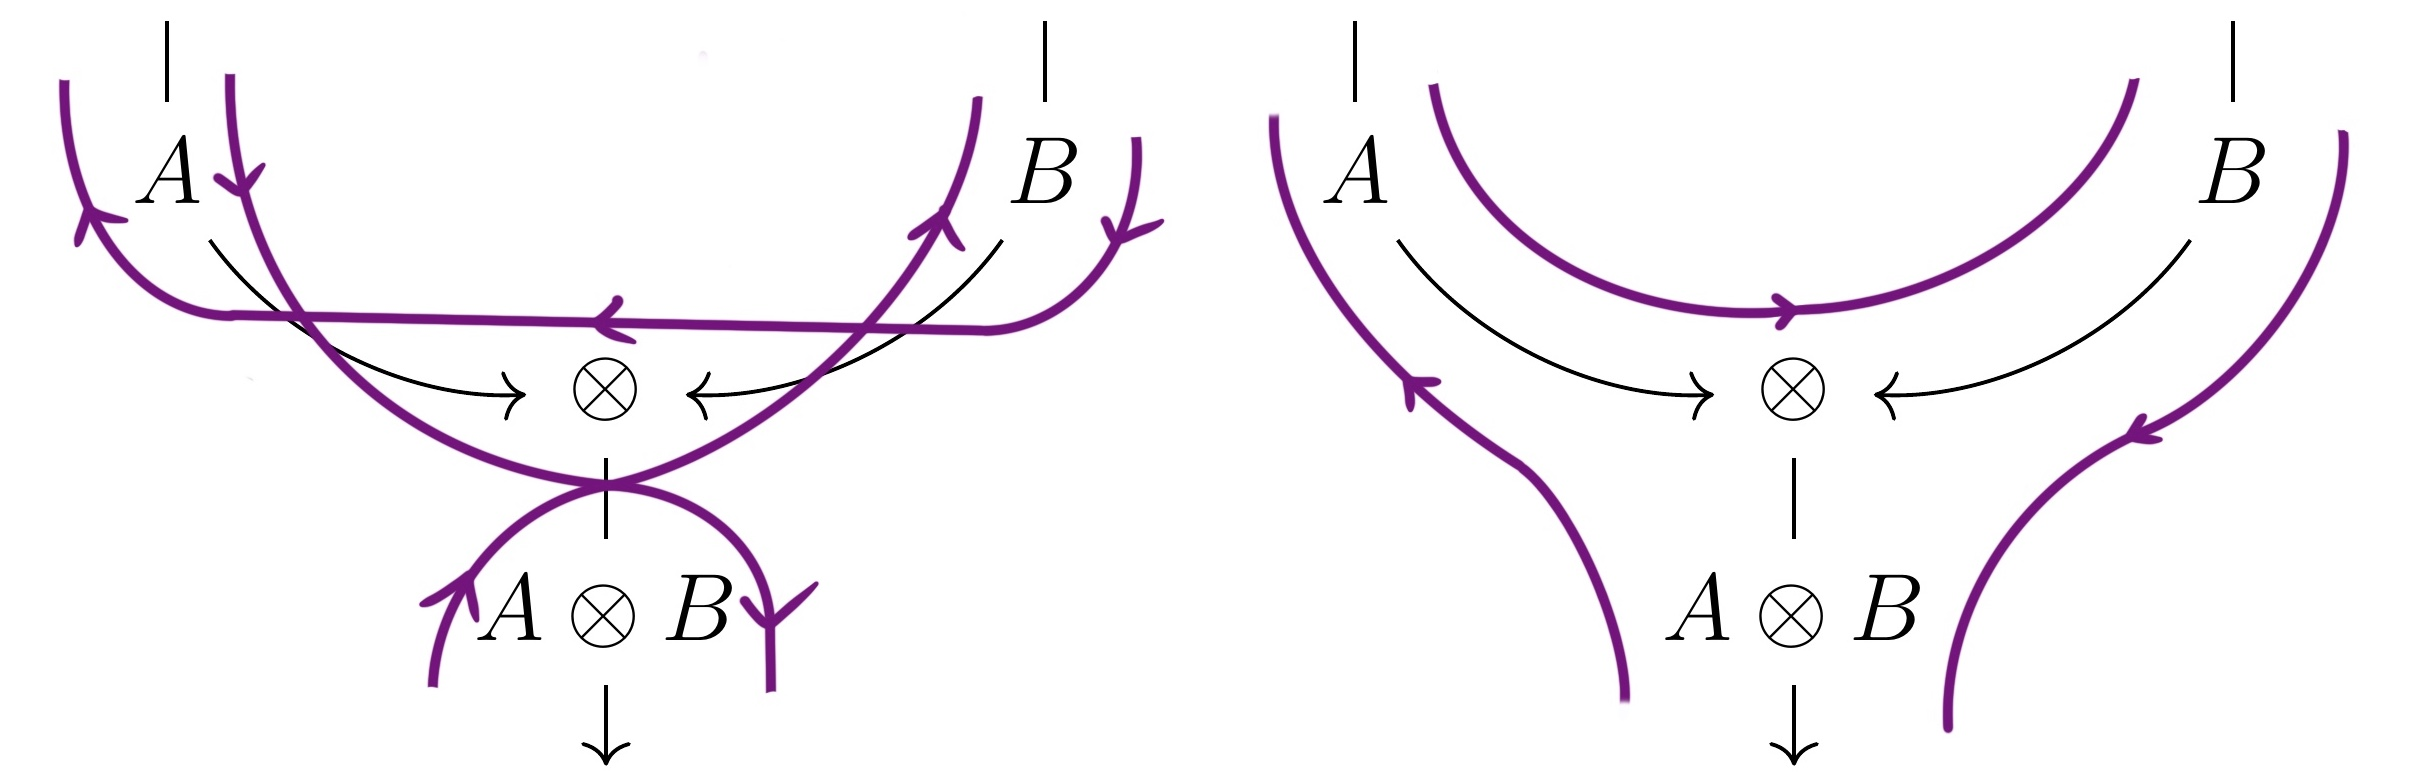
\includegraphics[width = 0.8\textwidth]{TensorSwitch.jpg}
		\caption{Tensor link, $L$ switching, $R$ switching}
		\label{fig:tensorswitching}
	\end{figure}
		\begin{figure}[h]
			\centering
			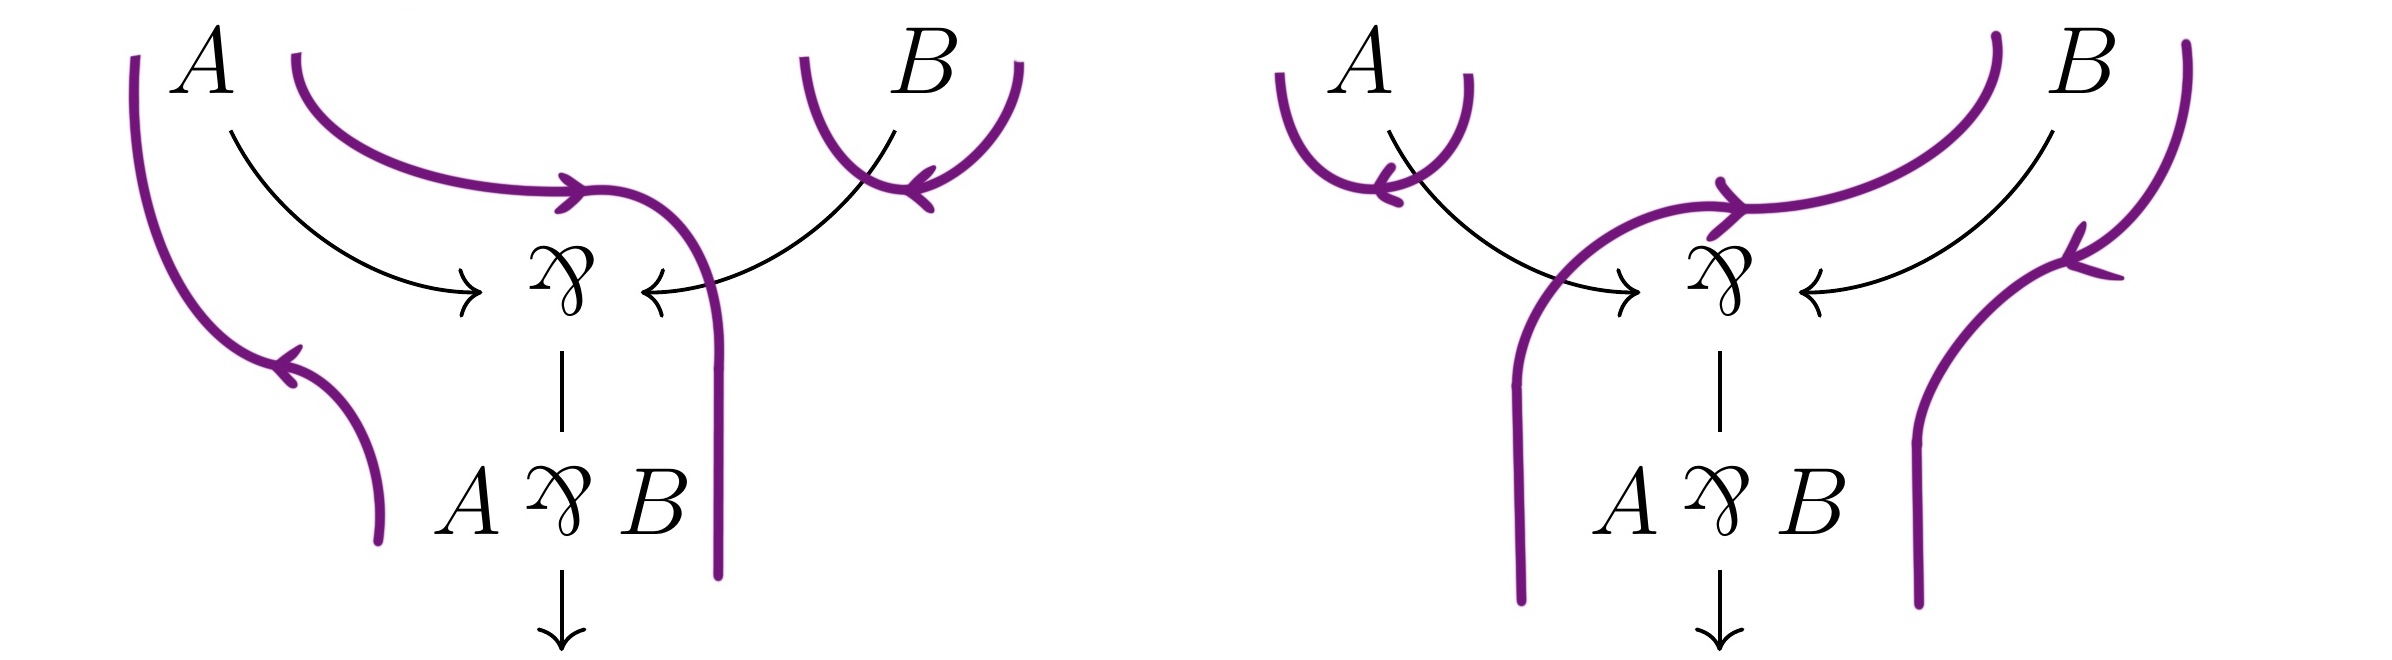
\includegraphics[width = 0.8\textwidth]{ParSwitch.jpg}
			\caption{Par link, $L$ switching, $R$ switching.}
			\label{fig:parrswitching}
		\end{figure}
		\begin{defn}
			Let $\operatorname{Pre}\call{T}(\pi,S)$ denote the set of all pretrips of $\pi$ with respect to $S$. We define an equivalence relation on this set $\sim$ where two pretrips $(x_1,...,x_n)$ and $(y_1,...,y_m)$ are equivalent if $n = m$, and there exists an integer $k$ such that $x_{i + k} = y_i$ (where $i + k$ means $\operatorname{mod} n$) for all $i = 1,...,n$.
			
			A \textbf{trip} of $\pi$ with respect to $S$ is an equivalence class of pretrips. We denote the set of all trips by $\call{T}(\pi,S)$.  If the set $\call{T}(\pi,S)$ admits more than one element, these elements are called \textbf{short trips}, and if it admits only one element, this element is the \textbf{long trip}. We refer to the statement ``for all switchings $S$, the set $\call{T}(\pi,S)$ contains exactly one element" as the \textbf{long trip condition}.
			
			A \textbf{short pretrip} is a choice of representative for a pretrip, and a \textbf{long pretrip} is a choice of representatitive of a long trip.
		\end{defn}
		
	\end{defn}
	Given a proof structure $\pi$ satisfying the long trip condition and a tensor link $l$ with premises $A,B$ say, let $S$ be a switching of $\pi$ and $t := (x_1,...,x_n)$ be the long pretrip of $\pi$ satisfying $x_1 =A\downarrow$. Since $\pi$ satisfies the long trip condition, it must be the case that $\uparrow (A \otimes B)$ and $B\downarrow$ occur somewhere in $t$, can we determine which occurs earlier? Let $m,l > 0$ be such that $x_m = \uparrow (A \otimes B), x_l = B\downarrow$ and assume $l < m$. Say $S(\tau) = L$, then $t$ has the shape
	\begin{equation}\label{eq:sequence_left_switch_tensor}
		(A\downarrow, (A \otimes B)\downarrow, ..., B \downarrow, \uparrow A, ..., \uparrow (A \otimes B), \uparrow B, ..., A\downarrow)
	\end{equation}
	Now consider the switching given by
	\[\hat{S}(\sigma) = \begin{cases}
		S(\sigma),& \sigma \neq \tau\\
		R, & \sigma = \tau
	\end{cases}
	\]
	Then \eqref{eq:sequence_left_switch_tensor} becomes:
	\begin{equation}
		(A\downarrow, \uparrow B, ..., A\downarrow)
	\end{equation}
	which is a short pretrip, contradicting the assumption that $\pi$ satisfies the long trip condition. Thus $m < l$. We have proven (the first half) of the following.
	\begin{lemma}\label{lem:stays_contained_tensor}
		Let $\pi$ be a proof structure satisfying the long trip condition, $l$ be a tensor link with premises $A,B$ say, $S$ be a switching of $\pi$ and $(x_1,...,x_n)$ the long pretrip satisfying $x_1 = A \downarrow$. If $m,l > 0$ are such that $x_m = \uparrow (A \otimes B), x_l = B \downarrow$, then:
		\begin{itemize}
			\item if $S(\tau) = L$ then $m < l$,
			\item if $S(\tau) = R$ then $l < m$.
		\end{itemize}
	\end{lemma}
	The proof of the other half is similar to what has already been written, however since Lemma \ref{lem:stays_contained_tensor} contradicts \cite[Lemma 2.9.1]{linearlogic} we write out the details here:
	\begin{proof}
		Say $m < l$, then $t$ has the shape
		\begin{equation}\label{eq:sequence_right_switch_tensor}
			(A\downarrow, \uparrow B, ..., \uparrow (A \otimes B), \uparrow A, ..., B \downarrow, (A \otimes B)\downarrow, ..., A\downarrow)
		\end{equation}
		Now consider the switching given by
		\[
		S'(\sigma) = 
		\begin{cases}
			S(\sigma),& \sigma \neq \tau\\
			L, & \sigma = \tau
		\end{cases}
		\]
		Then \eqref{eq:sequence_right_switch_tensor} becomes:
		\begin{equation}
			(A\downarrow, (A \otimes B)\downarrow,..., A\downarrow)
		\end{equation}
		which is a short pretrip.
	\end{proof}
	\begin{lemma}\label{lem:stays_contained_par}
		Let $\pi$ be a proof structure satisfying the long trip condition, $l$ be a par link with premises $A,B$ say, $S$ be a switching of $\pi$ and $(x_1,...,x_n)$ be the long pretrip satisfying $x_1 = A\downarrow$. If $m,l > 0$ are such that $x_m = \uparrow (A \parr B), x_l = B\downarrow$, then
		\begin{itemize}
			\item if $S(\tau) = L$ then $m < l$,
			\item if $S(\tau) = R$ then $l < m$
		\end{itemize}
	\end{lemma}
	\begin{remark}
		Lemma \ref{lem:stays_contained_tensor} gives a nice interpretation of Lemma \ref{lem:stays_contained_tensor} that long trips \emph{return to where they left} at each tensor link.
		
		The situation is a bit different for par links; the relevant slogan is long tripes \emph{visit the premises before returning to the conclusion}.
	\end{remark}
	Say $\pi$ satisfies the long trip condition and moreover $\pi$ admits a tensor link $l$ (with premises $A,B$ say) such that if $l$ is removed, the resulting proof structure consists of two disjoint proof structures $\pi_1,\pi_2$ each satisfying the long trip condition. It is necessarily the case that any pretrip $\rho$ of $\pi$ starting at $\uparrow A$ visits the entirety of $\call{U}(\pi_1)$ before returning to the tensor link $l$, lest $\pi_1$ admit a short trip. Moreover, it must be the case that $\sigma$ admits no occurrence of formulas in $\pi_2$ lest the result of removing the tensor link $l$ not result in disjoint proof structures. Thus, if such a link $l$ exists, it is \emph{maximal} in the sense that there is no other tensor link $l'$ where a pretrip starting at a premise of $l'$ contains the entirety of any pretrip starting at $A$. The remainder of this Section will amount to proving the converse, that any such maximal tensor link ``splits" $\pi$.
	\begin{defn}\label{def:pretrip_from_A}
		Let $\pi$ be a proof structure satisfying the long trip condition, $S$ a switching of $\pi$, and $A$ an occurrence of a formula in $\pi$. Consider the long pretrip $(x_1,...,x_n)$ satisfying $x_1 = \uparrow A$. We denote by
		\begin{equation}
			\operatorname{PTrip}(\pi,S,A,\uparrow)
		\end{equation}
		the subsequence $(x_1,...,x_m)$ of $(x_1,...,x_n)$ satisfying $x_m = A\downarrow$. We define
		\begin{equation}
			\operatorname{PTrip}(\pi, S, A, \downarrow)
		\end{equation}
		similarly.
		
		Also, for $a \in \lbrace \uparrow,\downarrow\rbrace $ we define the following set
		\begin{equation}
			\operatorname{Visit}_S(A,a) := \lbrace C \in \call{O}(\pi) \mid \uparrow C, C\downarrow \text{ occur in } \operatorname{PTrip}(\pi,S,A,a)\rbrace
		\end{equation}
		The \textbf{up empire of $A$} is the following set:
		\begin{equation}
			\operatorname{Emp}_{\uparrow}A := \lbrace C \in \call{O}(\pi) \mid \text{For all switchings }S\text{ we have } \uparrow C, C\downarrow \text{ occur in } \operatorname{PTrip}(\pi,S, A,\uparrow)\rbrace
		\end{equation}
		The \textbf{down empire of $A$} is defined symmetrically.
	\end{defn}
	With this new terminology we now have some corollaries of Lemmas \ref{lem:stays_contained_tensor} and \ref{lem:stays_contained_par}:
	\begin{cor}\label{cor:pretrip_innards}
		Let $\pi$ be a proof structure satisfying the long trip condition, and let $S$ be a switching of $\pi$, for a formula $A$ and $a \in \lbrace \uparrow, \downarrow\rbrace$, denote $\operatorname{PTrip}(\pi,S, A, a)$ by $\operatorname{PTrip}(A,a)$:
		\begin{enumerate}
			\item if $A$ is part of an axiom link then
			\begin{equation}
				\operatorname{PTrip}(A,\uparrow) = \uparrow A, \operatorname{PTrip}(\negation A, \downarrow), A \downarrow
			\end{equation}
			\item if $l$ is a tensor link with conclusion $A \otimes B$:
			\begin{enumerate}
				\item if $S(l) = L$:
				\begin{equation}
					\operatorname{Ptrip}(A, \downarrow) = A\downarrow, \operatorname{PTrip}(A \otimes B, \downarrow), \operatorname{PTrip}(B, \uparrow), \uparrow A
				\end{equation}
				\begin{equation}
					\operatorname{PTrip}(B, \downarrow) = B\downarrow, \operatorname{PTrip}(A,\uparrow), \operatorname{PTrip}(A \otimes B, \downarrow), \uparrow B
				\end{equation}
				\begin{equation}
					\operatorname{PTrip}(A \otimes B, \uparrow) = \uparrow A \otimes B, \operatorname{PTrip}(B, \uparrow), \operatorname{PTrip}(A,\uparrow), A \otimes B \downarrow
				\end{equation}
				\item if $S(l) = R$:
				\begin{equation}
					\operatorname{PTrip}(A, \downarrow) = A\downarrow, \operatorname{PTrip}(B, \uparrow),\operatorname{PTrip}(A \otimes B, \downarrow), \uparrow A
				\end{equation}
				\begin{equation}
					\operatorname{PTrip}(B, \downarrow) = B\downarrow,  \operatorname{PTrip}(A \otimes B, \downarrow), \operatorname{PTrip}(A,\uparrow),\uparrow B
				\end{equation}
				\begin{equation}
					\operatorname{PTrip}(A \otimes B, \uparrow) = \uparrow A \otimes B,  \operatorname{PTrip}(A,\uparrow), \operatorname{PTrip}(B, \uparrow),A \otimes B \downarrow
				\end{equation}
			\end{enumerate}
			\item if $A$ is a premise of a par link $l$ with conclusion $A \parr B$:
			\begin{enumerate}
				\item if $S(l) = L$:
				\begin{equation}
					\operatorname{PTrip}(A,\downarrow) = A\downarrow, \operatorname{PTrip}(A \parr B, \downarrow), \uparrow A
				\end{equation}
				\begin{equation}
					\operatorname{PTrip}(B, \downarrow) = B\downarrow, \uparrow B
				\end{equation}
				\begin{equation}
					\operatorname{PTrip}(A \parr B, \uparrow) = \uparrow A \parr B, \operatorname{PTrip}(A, \uparrow), A \parr B \downarrow
				\end{equation}
				\item if $S(l) = R$:
				\begin{equation}
					\operatorname{PTrip}(A,\downarrow) = A\downarrow, \uparrow A
				\end{equation}
				\begin{equation}
					\operatorname{PTrip}(B, \downarrow) = B\downarrow, \operatorname{PTrip}(A \parr B, \downarrow), \uparrow B
				\end{equation}
				\begin{equation}
					\operatorname{PTrip}(A \parr B, \uparrow) = \uparrow A \parr B, \operatorname{PTrip}(B, \uparrow), A \parr B \downarrow
				\end{equation}
			\end{enumerate}
		\end{enumerate}
	\end{cor}
	In particular:
	\begin{cor}\label{cor:stays_contained_corollary}
		For any formula $A$ which is a premise to either a tensor or par link, and any $a \in \lbrace \uparrow, \downarrow \rbrace$, we have: $$\uparrow C \text{ occurs in } \operatorname{PTrip}(\pi,S,A,\uparrow)\qquad\text{ if and only if }\qquad C\downarrow \text{ occurs in } \operatorname{PTrip}(\pi,S,A,\downarrow)$$ and similarly for $\operatorname{PTrip}(\pi,S,A,\downarrow)$.
	\end{cor}
	\begin{proof}
		By induction on the length of the sequence $\operatorname{PTrip}(\pi,S,A,a)$ and appealing to Corollary \ref{cor:pretrip_innards}.
	\end{proof}
	\begin{cor}\label{cor:empire_features}
		Let $\pi$ be a proof structure satisfying the long trip condition,
		we have the following.
		\begin{enumerate}
			\item\label{cor:empire_features_up_ax} For any axiom link with conclusions $A, \neg A$:
			\begin{equation}
				\operatorname{Emp}_{\uparrow}A = \operatorname{Emp}_{\downarrow}(\neg A) \cup \lbrace A \rbrace
			\end{equation}
			\item\label{cor:empire_features_down_cut} For any cut link with premises $A, \neg A$:
			\begin{equation}
				\operatorname{Emp}_{\downarrow}A = \operatorname{Emp}_{\uparrow}(\neg A) \cup \lbrace A \rbrace
			\end{equation}
			\item\label{cor:empire_features_empty_int} For any tensor link with premises $A,B$:
			\begin{equation}
				\operatorname{Emp}_{\uparrow}A \cap \operatorname{Emp}_{\uparrow}B = \varnothing
			\end{equation}
			\item\label{cor:empire_features_up_tens_par} For any tensor or par link with premises $A,B$ and conclusion $C$:
			\begin{equation}
				\operatorname{Emp}_{\uparrow}C = \operatorname{Emp}_{\uparrow}A \cup \operatorname{Emp}_{\uparrow}B \cup \lbrace C \rbrace
			\end{equation}
			\item\label{cor:empire_features_down_tens} For any tensor link with premises $A,B$:
			\begin{equation}
				\operatorname{Emp}_{\downarrow}B = \operatorname{Emp}_{\uparrow}A \cup \operatorname{Emp}_{\downarrow}(A \otimes B) \cup \lbrace B \rbrace
			\end{equation}
			and similarly:
			\begin{equation}
				\operatorname{Emp}_{\downarrow}A = \operatorname{Emp}_{\uparrow}B \cup \operatorname{Emp}_{\downarrow}(A \otimes B) \cup \lbrace A\rbrace
			\end{equation}
		\end{enumerate}
	\end{cor}
	\begin{defn}
		Given any link $l$ we write $B \in l$ if $B$ occurs as either a premise or a conclusion of $l$.
		
		Let $\pi$ be a proof structure satisfying the long trip condition, and $a \in \lbrace \uparrow, \downarrow\rbrace$. The set of \textbf{links of $A$ with respect to $S$} is the set
		\begin{equation}
			\operatorname{Link}_aA := \lbrace l \in \operatorname{Link}\pi \mid \forall B \in l, B \in \operatorname{Emp}_aA \rbrace
		\end{equation}
	\end{defn}
	\begin{defn}
		Let $\pi$ be a proof structure satisfying the long trip condition and let $a \in \lbrace \uparrow, \downarrow \rbrace$. Define the set
		\begin{equation}
			\operatorname{Link}^0_{\parr,a}A := \lbrace l \in \operatorname{Link}\pi \mid \text{Exactly one premise of }l\text{ is in }\operatorname{Emp}_{a}A\rbrace
		\end{equation}
	\end{defn}
	\begin{lemma}[Realisation Lemma]\label{lem:realisation_switching}
		Let $\pi$ be a cut-free proof structure satisfying the long trip condition, let $a \in \lbrace \uparrow, \downarrow \rbrace$ and $A$ an occurrence of a formula in $\pi$. Define the following function:
		\begin{align*}
			S: \operatorname{Link}_{\parr,a}^0A &\lto \lbrace L,R\rbrace\\
			l &\longmapsto
			\begin{cases}
				L, & \text{if the right premise of }l\text{ is in }\operatorname{Emp}_{a}A\\
				R, & \text{if the left premise of }l\text{ is in }\operatorname{Emp}_{a}A
			\end{cases}
		\end{align*}
		and extend this to a switching $\hat{S}: \operatorname{Link}\pi \lto \lbrace L,R \rbrace$ arbitrarily. Then
		\begin{equation}
			\operatorname{Emp}_aA = \operatorname{Visit}_{\hat{S}}(A,a)
		\end{equation}
	\end{lemma}
	\begin{proof}
		We proceed by induction on the size $|\operatorname{Link}_a(A)|$ of the set $\operatorname{Link}_a(A)$. For the base case, assume $|\operatorname{Link}_a(A)| = 0$. The formula $A$ is part of an axiom link and so $\operatorname{Emp}_{\uparrow}A = A, \negation A$ and $\operatorname{Emp}_{\downarrow}A = A$, the result follows easily.
		
		Now assume that $|\operatorname{Link}_a A| = n > 0$ and the result holds for any formula $B$ such that $|\operatorname{Link}_aB| < n$. First say $a = \uparrow$, and $A$ is a conclusion of either a tensor or a par link
		% https://q.uiver.app/?q=WzAsNSxbMCwwLCJBXzEiXSxbMiwwLCJBXzIiXSxbMSwxLCJcXGJveHRpbWVzIl0sWzEsMiwiQSJdLFsxLDMsIlxcdmRvdHMiXSxbMyw0XSxbMSwyLCIiLDAseyJjdXJ2ZSI6LTIsInN0eWxlIjp7ImhlYWQiOnsibmFtZSI6Im5vbmUifX19XSxbMCwyLCIiLDIseyJjdXJ2ZSI6Miwic3R5bGUiOnsiaGVhZCI6eyJuYW1lIjoibm9uZSJ9fX1dLFsyLDNdXQ==
		\[\begin{tikzcd}
			{A_1} && {A_2} \\
			& \boxtimes \\
			& A \\
			& \vdots
			\arrow[from=3-2, to=4-2]
			\arrow[curve={height=-12pt}, no head, from=1-3, to=2-2]
			\arrow[curve={height=12pt}, no head, from=1-1, to=2-2]
			\arrow[from=2-2, to=3-2]
		\end{tikzcd}\]
		where $\boxtimes \in \lbrace \otimes, \parr \rbrace$ and $A = A_1 \otimes A_2$ or $A = A_1 \parr A_2$. By \eqref{cor:empire_features_up_tens_par} we have
		\begin{align*}
			\operatorname{Emp}_{\uparrow}A &= \operatorname{Emp}_{\uparrow}A_1 \cup \operatorname{Emp}_{\uparrow}A_2 \cup \lbrace A\rbrace\\
			&= \operatorname{Visit}_{\hat{S}}(A_1,\uparrow) \cup \operatorname{Visit}_S(A_2,\uparrow) \cup \lbrace A \rbrace\\
			&= \operatorname{Visit}_{\hat{S}}(A, \uparrow)
		\end{align*}
		where the second equality follows from the inductive hypothesis.
		
		Assume $A$ is part of an axiom link. By \eqref{cor:empire_features_up_ax}
		\begin{equation}
			\operatorname{Emp}_{\uparrow}A = \operatorname{Emp}_{\downarrow}(\neg A) \cup \lbrace A \rbrace
		\end{equation}
		with
		\begin{equation}
			|\operatorname{Link}_{\uparrow}A| = |\operatorname{Link}_{\downarrow}(\neg A)|
		\end{equation}
		Since $|\operatorname{Link}_{\downarrow}(\negation A)| > 0$ we necessarily have that $\negation A$ is not a conclusion. Thus, since $\pi$ is cut-free, $A$ is connected to an occurrence $\negation A$ which is a premise to either a tensor link or a par link. In the case of the former, we have:
		% https://q.uiver.app/?q=WzAsNSxbMCwwLCJDIl0sWzIsMCwiXFxuZWcgQSJdLFsxLDEsIlxcb3RpbWVzIl0sWzEsMiwiQyBcXG90aW1lcyBcXG5lZyBBIl0sWzEsMywiXFx2ZG90cyJdLFszLDRdLFsxLDIsIiIsMCx7ImN1cnZlIjotMiwic3R5bGUiOnsiaGVhZCI6eyJuYW1lIjoibm9uZSJ9fX1dLFswLDIsIiIsMix7ImN1cnZlIjoyLCJzdHlsZSI6eyJoZWFkIjp7Im5hbWUiOiJub25lIn19fV0sWzIsM11d
		\[\begin{tikzcd}[column sep = small, row sep = small]
			C && {\neg A} \\
			& \otimes \\
			& {C \otimes \neg A} \\
			& \vdots
			\arrow[from=3-2, to=4-2]
			\arrow[curve={height=-12pt}, no head, from=1-3, to=2-2]
			\arrow[curve={height=12pt}, no head, from=1-1, to=2-2]
			\arrow[from=2-2, to=3-2, no head]
		\end{tikzcd}\]
		then by \eqref{cor:empire_features_down_tens}:
		\begin{align*}
			\operatorname{Emp}_{\downarrow}(\neg A) &= \operatorname{Emp}_{\uparrow}C \cup \operatorname{Emp}_{\downarrow}(C \otimes \neg A) \cup \lbrace \neg A\rbrace\\
			&= \operatorname{Visit}_{\hat{S}}(C,\uparrow) \cup \operatorname{Visit}_{\hat{S}}(C \otimes \neg A,\downarrow) \cup \lbrace \neg A\rbrace\\
			&= \operatorname{Visit}_{\hat{S}}(\neg A, \downarrow)
		\end{align*}
		where the second equality follows from the inductive hypothesis.
		
		If $\negation A$ is a premise of a par link
		\[\begin{tikzcd}[column sep = small, row sep = small]
			C && {\neg A} \\
			& \parr \\
			& {C \parr \neg A} \\
			& \vdots
			\arrow[from=3-2, to=4-2]
			\arrow[curve={height=-12pt}, no head, from=1-3, to=2-2]
			\arrow[curve={height=12pt}, no head, from=1-1, to=2-2]
			\arrow[from=2-2, to=3-2, no head]
		\end{tikzcd}\]
		then by construction of $\hat{S}$, where we use the specific definition of $S$ for the first time,
		\begin{align*}
			\operatorname{Emp}_{\downarrow}(\neg A) &= \lbrace \neg A\rbrace\\
			&= \operatorname{Visit}_{\hat{S}}(\neg A,\downarrow)
		\end{align*}
		The case when $a = \downarrow$ is exactly similar and so we omit the proof.
	\end{proof}
	\begin{defn}
		A tensor or par link is \textbf{terminal} if it is a conclusion.
	\end{defn}
	\begin{cor}\label{lem:par_link_existence}
		Let $\pi$ be a cut-free proof structure satisfying the long trip condition. Let
		\[l = \begin{tikzcd}[column sep = small, row sep = small]
			A && {B} \\
			& \otimes \\
			& {A \otimes B} \\
			& \operatorname{c}
			\arrow[from=3-2, to=4-2]
			\arrow[curve={height=-12pt}, no head, from=1-3, to=2-2]
			\arrow[curve={height=12pt}, no head, from=1-1, to=2-2]
			\arrow[from=2-2, to=3-2, no head]
		\end{tikzcd}\]
		be a terminal tensor link of $\pi$. Then $\pi$ admits a par link
		\[l' := \begin{tikzcd}[column sep = small, row sep = small]
			C && {D} \\
			& \otimes \\
			& {C \parr D} \\
			& \vdots
			\arrow[from=3-2, to=4-2]
			\arrow[curve={height=-12pt}, no head, from=1-3, to=2-2]
			\arrow[curve={height=12pt}, no head, from=1-1, to=2-2]
			\arrow[from=2-2, to=3-2, no head]
		\end{tikzcd}\]
		such that either $C \in \operatorname{Emp}_{\uparrow}A$ and $D \in \operatorname{Emp}_{\uparrow}B$ or $C \in \operatorname{Emp}_{\uparrow}B$ and $D \in \operatorname{Emp}_{\uparrow}A$ if and only if for any switching $S$ of $\pi$ we have that either
		\[\operatorname{Emp}_{\uparrow}A \subsetneq \operatorname{Visit}_S(A,\uparrow)\qquad\text{or}\qquad \operatorname{Emp}_{\uparrow}B \subsetneq \operatorname{Visit}_S(B,\uparrow)\]
	\end{cor}
	\begin{proof}
		Say $\pi$ admitted $l'$ and $C \in \operatorname{Emp}_{\uparrow}A$ and $D \in \operatorname{Emp}_{\uparrow}B$. If the switching $S$ is such that $S(l) = L$ then $C \parr D \in \operatorname{Visit}_S(B)\setminus \operatorname{Emp}_{\uparrow}B$ and if $S(\tau) = R$ then $C \parr D \in \operatorname{Visit}_S(A) \setminus \operatorname{Emp}_{\uparrow}A$. The other case is similar.
		
		Conversely, say $\pi$ admits no such par link $l'$, that is, assume
		\begin{equation}
			\operatorname{Link}^0_{\parr,\uparrow}(A) \cap \operatorname{Link}^0_{\parr,\uparrow}(B) = \varnothing
		\end{equation}
		Then there is by Lemma \ref{lem:realisation_switching} a well defined function $$S: \operatorname{Link}_{\parr,\uparrow}^0(A) \cup \operatorname{Link}^0_{\parr,\uparrow}(B) \lto \lbrace L, R \rbrace$$ which extends to a switching $\hat{S}$ such that
		\begin{equation}
			\operatorname{Emp}_{\uparrow}A = \operatorname{Visit}_{\hat{S}}(A,\uparrow)\qquad\text{and}\qquad \operatorname{Emp}_{\uparrow}B = \operatorname{Visit}_{\hat{S}}(B,\uparrow)
		\end{equation}
	\end{proof}
	
	\begin{lemma}[Separation Lemma]
		A cut-free proof structure $\pi$ satisfying the long trip condition, with only tensor links amongst its conclusions admits a tensor link
		\[l := \begin{tikzcd}[column sep = small, row sep = small]
			A && {B} \\
			& \otimes \\
			& {A \otimes B} \\
			& \operatorname{c}
			\arrow[from=3-2, to=4-2]
			\arrow[curve={height=-12pt}, no head, from=1-3, to=2-2]
			\arrow[curve={height=12pt}, no head, from=1-1, to=2-2]
			\arrow[from=2-2, to=3-2, no head]
		\end{tikzcd}\]
		satisfying
		\begin{equation}
			\call{O}(\pi) = \operatorname{Emp}_{\uparrow}A \cup \operatorname{Emp}_{\uparrow}B \cup \lbrace A \otimes B\rbrace
		\end{equation}
		Moreover, removing $A \otimes B$ results in a disconnected graph with each component a proof structure satisfying the long trip condition.
	\end{lemma}
	\begin{proof}
		Consider the set of tensor links $\operatorname{Link}_{\otimes}(\pi)$ of $\pi$. We endow this with the following partial order $\leq$: a pair of links:
		\[
		l' := \begin{tikzcd}[column sep = small, row sep = small]
			A && {B} \\
			& \otimes \\
			& {A \otimes B} \\
			& \vdots
			\arrow[from=3-2, to=4-2]
			\arrow[curve={height=-12pt}, no head, from=1-3, to=2-2]
			\arrow[curve={height=12pt}, no head, from=1-1, to=2-2]
			\arrow[from=2-2, to=3-2, no head]
		\end{tikzcd}
		%
		\qquad
		%
		l'' :=
		\begin{tikzcd}[column sep = small, row sep = small]
			C && {D} \\
			& \otimes \\
			& {C \otimes D} \\
			& \vdots
			\arrow[from=3-2, to=4-2]
			\arrow[curve={height=-12pt}, no head, from=1-3, to=2-2]
			\arrow[curve={height=12pt}, no head, from=1-1, to=2-2]
			\arrow[from=2-2, to=3-2, no head]
		\end{tikzcd}
		\]
		are such that $l' \leq l''$ if $\operatorname{Emp}_{\uparrow}A \cup \operatorname{Emp}_{\uparrow}B \subseteq \operatorname{Emp}_{\uparrow}C \cup \operatorname{Emp}_{\uparrow}D$. Let $l$ (with conclusion $A \otimes B$ say) be a tensor link maximal with respect to $\leq$. We show that $l$ satisfies the required property.
		
		Say $\call{O}(\pi) \neq \operatorname{Emp}_{\uparrow}A \cup \operatorname{Emp}_{\uparrow}B \cup \lbrace A \otimes B\rbrace$. Then by Lemma \ref{lem:par_link_existence} there exists a par link
		\[
		l' = \begin{tikzcd}[column sep = small, row sep = small]
			C && {D} \\
			& \parr \\
			& {C \parr D} \\
			& \vdots
			\arrow[from=3-2, to=4-2]
			\arrow[curve={height=-12pt}, no head, from=1-3, to=2-2]
			\arrow[curve={height=12pt}, no head, from=1-1, to=2-2]
			\arrow[from=2-2, to=3-2, no head]
		\end{tikzcd}
		\]
		such that either $C \in \operatorname{Emp}_{\uparrow}A$ and $D \in \operatorname{Emp}_{\uparrow}B$ or $C \in \operatorname{Emp}_{\uparrow}B$ and $D \in \operatorname{Emp}_{\uparrow}A$. We show the proof in the case of the former. Since $\pi$ admits no terminal par links, this link is above a tensor link
		\[l'':= \begin{tikzcd}[column sep = small, row sep = small]
			E && {F} \\
			& \otimes \\
			& {E \otimes F} \\
			& \vdots
			\arrow[from=3-2, to=4-2]
			\arrow[curve={height=-12pt}, no head, from=1-3, to=2-2]
			\arrow[curve={height=12pt}, no head, from=1-1, to=2-2]
			\arrow[from=2-2, to=3-2, no head]
		\end{tikzcd}\]
		Notice that if $l'' = l$, then either $C \parr D \in \operatorname{Emp}_{\uparrow}A$ or $C \parr D \in \operatorname{Emp}_{\uparrow}B$ which in either case implies $\operatorname{Emp}_{\uparrow}A \cap \operatorname{Emp}_{\uparrow}B \neq \varnothing$, contradicting Corollary \ref{cor:empire_features}, \ref{cor:empire_features_empty_int}, and so $l'' \neq l$. Without any loss of generality, assume that $\sigma$ sits above $F$. Let $S$ be a switching of $\pi$ so that $\operatorname{Emp}_{\uparrow}F = \operatorname{Visit}_S(F,\uparrow)$ and so that $S(l') = L$, which exists by Lemma \ref{lem:par_link_existence}. Let $t = (x_1,...,x_n)$ be the long pretrip of $\pi$ with respect to $S$ satisfying $x_1 = F\uparrow$. We have by Lemma \ref{lem:stays_contained_par} that $t$ takes the following shape:
		\begin{equation}\label{eq:condemning_shape}
			\uparrow F, ..., \uparrow(C \parr D), \uparrow C, ..., D\downarrow, \uparrow D, ..., C\downarrow, (C \parr D)\downarrow, ..., F\downarrow,...
		\end{equation}
		We have that $D \in \operatorname{Emp}_{\uparrow}B$ so for simplicity, rewrite \eqref{eq:condemning_shape} as $t' = (x_{1 + k},...,x_{n+k})$ for some $k > 0$ (where $i + k$ means $i + k\operatorname{mod} n$) so that $t$ takes the shape
		\begin{equation}\label{eq:condemning_shape_altered}
			..., \uparrow F, ..., \uparrow(C \parr D), \uparrow C, ..., D\downarrow, \uparrow D, ..., C\downarrow, (C \parr D)\downarrow, ..., F\downarrow,...
		\end{equation}
		with $\uparrow B$ occurring to the left of $D \downarrow$ and $B \downarrow$ occurring to the right of $\uparrow D$.
		We have that $C \not\in \operatorname{Emp}_{\uparrow}B$ and so by Corollary \ref{cor:stays_contained_corollary}:
		\begin{equation}
			\uparrow B \text{ occurrs in }\uparrow C,..., D\downarrow\text{ and } B\downarrow\text{ occurrs in }\uparrow D, ..., C\downarrow
		\end{equation}
		However, this implies that $B \in \operatorname{Visit}_S(F,\uparrow)$ which by Lemma \ref{lem:realisation_switching} implies $B \in \operatorname{Emp}_{\uparrow}F$.
		
		By reversing the switching of $l'$ and interchanging the rolls of $C,D$ in the above argument, we also have that $A \in \operatorname{Emp}_{\uparrow}F$, contradicting the maximality of $l$. This proves the first claim.
		
		For the second claim, since $\call{O}(\pi) = \operatorname{Emp}_{\uparrow}A \cup \operatorname{Emp}_{\uparrow}B \cup \lbrace A \otimes B\rbrace$ we have by Lemma \ref{lem:par_link_existence} that
		\begin{equation}
			\operatorname{Link}_{\parr,\uparrow}^0(A\otimes B) = \varnothing
		\end{equation}
		and we saw in the proof of Lemma \ref{lem:realisation_switching} that a switching $S$ which realises $\operatorname{Emp}_{\uparrow}A$ is given by setting all switchings arbitrarily except for those in $\operatorname{Link}_{\parr,\uparrow}^0(A\otimes B)$. This means that for any switching $S$ of $\pi$:
		\begin{equation}
			\operatorname{Visit}_{S}(A,\uparrow) = \operatorname{Emp}_{\uparrow}A \qquad\text{and}\qquad \operatorname{Visit}_{S}(B,\uparrow) = \operatorname{Emp}_{\uparrow}B
		\end{equation}
		which is to say the two subproof structures given by removing $A \otimes B$ never admit a short trip, that is, they each satisfy the long trip condition.
	\end{proof}
	\begin{thm}[The Sequentialisation Theorem]\label{thm:sequentialisation}
		A proof structure $\pi$ (possibly with cuts) satisfies the long trip condition if and only $\pi$ is a proof net.
	\end{thm}
	\begin{proof}
		First assume that $\pi$ is cut-free.
		
		We proceed by induction on the size $|\operatorname{Link}\pi|$ of the set $\operatorname{Link}\pi$. If there this is zero then $\pi$ consists of a single axiom link and so the result is clear.
		
		For the inductive step, we consider two cases, first say $\pi$ admits a par link for a conclusion. Then removing this par link clearly results in two cut-free subproof structures satsifying the long trip condition and so the result follows from the inductive hypothesis. If no such terminal par link exists, then by the Separation Lemma there exists some tensor link in the conclusion for which we can remove and apply the inductive hypothesis.
		
		Now say that $\pi$ contained cuts. We replace each cut with a tensor link to create a new proof $\zeta$. That there exists a proof $\Xi$ which maps to $\zeta$ follows from the part of the result proved already as $\zeta$ is cut-free. We adapt $\Xi$ appropriately by replacing $\otimes$-rules by $\operatorname{cut}$-rules and we are done.
	\end{proof}
	\section{Proofs as permutations}
\begin{defn}
	Let $\pi$ be a proof net. Let $\call{P}(\pi)$ denote the disjoint union of all the unoriented axioms of all formulas which are conclusions to axiom links in $\pi$.
\end{defn}
\begin{example}\label{ex:permutation_example}
	Let $\pi$ denote the following proof net, where $X,Y$ are atomic. For simplicity, we usually attach artificial labels to the conclusions of axiom links. So, in the following example, for any integer $i$ and any $Z = X,Y$, the notation $Z_i$ simply means $Z$.
	% https://q.uiver.app/?q=WzAsMTEsWzAsMSwiKFggLCspIFxcb3RpbWVzIChZLC0pIl0sWzIsMSwiKFgsIC0pIFxccGFyciAoWSwrKSJdLFsxLDAsIlxcYXgiXSxbNSwwLCJcXGF4Il0sWzQsMSwiKFgsKykiXSxbNiwxLCIoWSwtKSJdLFszLDIsIlxcb3RpbWVzIl0sWzMsMywiKChYLC0pXFxwYXJyKFksKykpXFxvdGltZXMgKFgsKykiXSxbMCwyLCJcXG9wZXJhdG9ybmFtZXtjfSJdLFs2LDIsIlxcb3BlcmF0b3JuYW1le2N9Il0sWzMsNCwiXFxvcGVyYXRvcm5hbWV7Y30iXSxbMiwxLCIiLDAseyJjdXJ2ZSI6LTIsInN0eWxlIjp7ImhlYWQiOnsibmFtZSI6Im5vbmUifX19XSxbMiwwLCIiLDIseyJjdXJ2ZSI6Miwic3R5bGUiOnsiaGVhZCI6eyJuYW1lIjoibm9uZSJ9fX1dLFszLDQsIiIsMCx7ImN1cnZlIjoyLCJzdHlsZSI6eyJoZWFkIjp7Im5hbWUiOiJub25lIn19fV0sWzMsNSwiIiwyLHsiY3VydmUiOi0yLCJzdHlsZSI6eyJoZWFkIjp7Im5hbWUiOiJub25lIn19fV0sWzYsNywiIiwyLHsic3R5bGUiOnsiaGVhZCI6eyJuYW1lIjoibm9uZSJ9fX1dLFs0LDYsIiIsMSx7ImN1cnZlIjotMn1dLFsxLDYsIiIsMSx7ImN1cnZlIjoyfV0sWzcsMTBdLFs1LDldLFswLDhdXQ==
	\[\begin{tikzcd}[column sep = tiny, row sep = small]
		& \ax &&&& \ax \\
		{(X_1 ,+) \otimes (Y_2,-)} && {(X_3, -) \parr (Y_4,+)} && {(X_5,+)} && {(Y_6,-)} \\
		{\operatorname{c}} &&& \otimes &&& {\operatorname{c}} \\
		&&& {((X,-)\parr(Y,+))\otimes (X,+)} \\
		&&& {\operatorname{c}}
		\arrow[curve={height=-12pt}, no head, from=1-2, to=2-3]
		\arrow[curve={height=12pt}, no head, from=1-2, to=2-1]
		\arrow[curve={height=12pt}, no head, from=1-6, to=2-5]
		\arrow[curve={height=-12pt}, no head, from=1-6, to=2-7]
		\arrow[no head, from=3-4, to=4-4]
		\arrow[curve={height=-12pt}, from=2-5, to=3-4]
		\arrow[curve={height=12pt}, from=2-3, to=3-4]
		\arrow[from=4-4, to=5-4]
		\arrow[from=2-7, to=3-7]
		\arrow[from=2-1, to=3-1]
	\end{tikzcd}\]
Then:
\begin{equation}
	\call{P}(\pi) = \lbrace X \rbrace \coprod \lbrace Y \rbrace \coprod \lbrace X \rbrace \coprod \lbrace Y \rbrace \coprod \lbrace X \rbrace \coprod \lbrace Y \rbrace = \lbrace X_1,Y_2,X_3,Y_4,X_5,Y_6\rbrace
\end{equation}

\end{example}
\begin{defn}\label{def:seq_set}
	Let $A$ be a formula with sequence of oriented atoms $\big((X_1,x_1),...,(X_n,x_n)\big)$. The \textbf{sequence of unoriented atoms} of $A$ is $(X_1,...,X_n)$ and the \textbf{set of unoriented atoms} of $A$ is the disjoint union $\lbrace X_1 \rbrace \coprod \hdots \coprod \lbrace X_n \rbrace$.
\end{defn}
	\begin{defn}\label{def:permutations}
		Let $\pi$ be a proof net with axiom links $l_1,...,l_n$ say. For each $i = 1,...,n$ the link $l_i$ defines a permutation $\tau_{l_i}$ on the set $\call{P}(\pi)$ in the following way: if $l_i$ has conclusions $A, \neg A$ then the $j^\text{th}$ element of the sequence of unoriented atoms of $A$ is mapped via $\tau_{l_i}$ to the $j^\text{th}$ element of the sequence of unoriented atoms of $\neg A$. We define $\alpha_\pi$ to be the product of all these permutations.
		\begin{equation}
			\alpha_\pi := \tau_{l_1}\hdots \tau_{l_n}
		\end{equation}
		We call this permutation the \textbf{axiom link permutation associated to $\pi$}.
		
		There is another permutation on $\call{P}(\pi)$ defined symmetrically but where the cut links are considered rather than the axiom links. We denote this permutation $\gamma_\pi$.
		
		There is yet another permutation on $\call{P}(\pi)$. Let $S$ be a switching of $\pi$. For each unoriented axiom $X \in \call{P}(\pi)$, corresponding to the formula $A$ say, let $\beta_{\pi}^S(X)$ denote the unoriented axiom corresponding to the first occurrence in $\operatorname{PTrip}(\pi,S,A,\downarrow)$ (Definition \ref{def:pretrip_from_A}) of the form $\uparrow B$ where $B$ is a formula labelling a conclusion of an axiom link in $\pi$.
		
		The set of all premutations of the second form is denoted:
		\begin{equation}
			\Sigma(\pi) := \lbrace \beta_{\pi}^S \mid S\text{ is a switching of }\pi\rbrace
		\end{equation}
		We will often denote elements of $\beta_{\pi}^S \in \Sigma(\pi)$ simply by $\beta$.
	\end{defn}
\begin{example}
	Continuing with Example \ref{ex:permutation_example}, and using the artifical labels we attributed to the atomic formulas of conclusions, we have $\alpha_\pi = (13)(24)(56)$ and since $\pi$ admits no cut links we have $\gamma_\pi = \operatorname{id}_{\call{P}(\pi)}$.
	
	The set $\Sigma(\pi)$ is uninteresting so we consider a more complicated example. Before doing this though, we introduce a simple Lemma for the sake of easing notation.
\end{example}
\begin{lemma}\label{lem:pars_or_not}
	Let $\pi$ be a proof net with conclusions $A_1,...,A_n$ and let $\zeta$ be a proof net obtained by beginning with $\pi$ and in any order forming par links which connect all the conclusions $A_1,...,A_n$ so that $\zeta$ has conclusions $B_1,...,B_m$ where $m \leq n$ and each $B_i$ is constructed only by $\parr$ and a subset of the formulas $A_1,...,A_n$. Then $\Sigma(\pi) = \Sigma(\zeta)$.
\end{lemma}
\begin{proof}
	Easy proof by induction on the integer given by the number of par links in $\zeta$ minus the number of par links in $\pi$.
\end{proof}
\begin{example}\label{ex:counter}
	\begin{figure}[h]
		\centering
		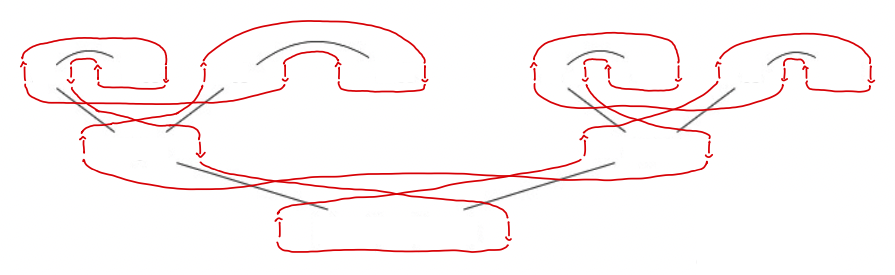
\includegraphics[width = 17cm]{Permutations.png}
		\caption{The set $\Sigma(\pi_1)$}
		\label{fig:counter_one}
	\end{figure}
	Let $\zeta$ be defined as follows, again, we explicitly place integer labells on the formulas, but $A_i$ denotes the formula $A$ for all $i$.
	% https://q.uiver.app/?q=WzAsMjMsWzAsMSwiQSJdLFsyLDEsIlxcbmVnIEEiXSxbMywxLCJBIl0sWzUsMSwiXFxuZWcgQSJdLFsyLDMsIlxcb3RpbWVzIl0sWzIsNCwiQSBcXG90aW1lcyBBIl0sWzEsMCwiXFxheCJdLFs0LDAsIlxcYXgiXSxbNiwxLCJBIl0sWzgsMSwiXFxuZWcgQSJdLFs5LDEsIkEiXSxbMTEsMSwiXFxuZWcgQSJdLFsxMCwwLCJcXGF4Il0sWzcsMCwiXFxheCJdLFs4LDMsIlxcb3RpbWVzIl0sWzgsNCwiQSBcXG90aW1lcyBBIl0sWzUsNSwiXFxvdGltZXMiXSxbNSw2LCIoQSBcXG90aW1lcyBBKSBcXG90aW1lcyAoQSBcXG90aW1lcyBBKSJdLFs1LDcsIlxcb3BlcmF0b3JuYW1le2N9Il0sWzIsMiwiXFxvcGVyYXRvcm5hbWV7Y30iXSxbNSwyLCJcXG9wZXJhdG9ybmFtZXtjfSJdLFs4LDIsIlxcb3BlcmF0b3JuYW1le2N9Il0sWzExLDIsIlxcb3BlcmF0b3JuYW1le2N9Il0sWzAsNCwiIiwwLHsiY3VydmUiOjJ9XSxbMiw0LCIiLDIseyJjdXJ2ZSI6LTJ9XSxbNCw1LCIiLDAseyJzdHlsZSI6eyJoZWFkIjp7Im5hbWUiOiJub25lIn19fV0sWzYsMCwiIiwwLHsiY3VydmUiOjIsInN0eWxlIjp7ImhlYWQiOnsibmFtZSI6Im5vbmUifX19XSxbNiwxLCIiLDIseyJjdXJ2ZSI6LTIsInN0eWxlIjp7ImhlYWQiOnsibmFtZSI6Im5vbmUifX19XSxbNywyLCIiLDIseyJjdXJ2ZSI6Miwic3R5bGUiOnsiaGVhZCI6eyJuYW1lIjoibm9uZSJ9fX1dLFs3LDMsIiIsMCx7ImN1cnZlIjotMiwic3R5bGUiOnsiaGVhZCI6eyJuYW1lIjoibm9uZSJ9fX1dLFsxMyw4LCIiLDAseyJjdXJ2ZSI6Miwic3R5bGUiOnsiaGVhZCI6eyJuYW1lIjoibm9uZSJ9fX1dLFsxMyw5LCIiLDIseyJjdXJ2ZSI6LTIsInN0eWxlIjp7ImhlYWQiOnsibmFtZSI6Im5vbmUifX19XSxbMTIsMTAsIiIsMix7ImN1cnZlIjoyLCJzdHlsZSI6eyJoZWFkIjp7Im5hbWUiOiJub25lIn19fV0sWzEyLDExLCIiLDAseyJjdXJ2ZSI6LTIsInN0eWxlIjp7ImhlYWQiOnsibmFtZSI6Im5vbmUifX19XSxbOCwxNCwiIiwwLHsiY3VydmUiOjJ9XSxbMTAsMTQsIiIsMix7ImN1cnZlIjotMn1dLFsxNCwxNSwiIiwyLHsic3R5bGUiOnsiaGVhZCI6eyJuYW1lIjoibm9uZSJ9fX1dLFs1LDE2LCIiLDAseyJjdXJ2ZSI6Mn1dLFsxNSwxNiwiIiwyLHsiY3VydmUiOi0yfV0sWzE2LDE3LCIiLDIseyJzdHlsZSI6eyJoZWFkIjp7Im5hbWUiOiJub25lIn19fV0sWzE3LDE4XSxbMSwxOV0sWzMsMjBdLFs5LDIxXSxbMTEsMjJdXQ==
	\[\begin{tikzcd}[column sep  = tiny, row sep = tiny]
		& \ax &&& \ax &&& \ax &&& \ax \\
		A_1 && {\neg A_2} & A_3 && {\neg A_4} & A_5 && {\neg A_6} & A_7 && {\neg A_8} \\
		&& {\operatorname{c}} &&& {\operatorname{c}} &&& {\operatorname{c}} &&& {\operatorname{c}} \\
		&& \otimes &&&&&& \otimes \\
		&& {A \otimes A} &&&&&& A \otimes A \\
		&&&&& \otimes \\
		&&&&& {(A \otimes A) \otimes (A \otimes A)} \\
		&&&&& {\operatorname{c}}
		\arrow[curve={height=12pt}, from=2-1, to=4-3]
		\arrow[curve={height=-12pt}, from=2-4, to=4-3]
		\arrow[no head, from=4-3, to=5-3]
		\arrow[curve={height=12pt}, no head, from=1-2, to=2-1]
		\arrow[curve={height=-12pt}, no head, from=1-2, to=2-3]
		\arrow[curve={height=12pt}, no head, from=1-5, to=2-4]
		\arrow[curve={height=-12pt}, no head, from=1-5, to=2-6]
		\arrow[curve={height=12pt}, no head, from=1-8, to=2-7]
		\arrow[curve={height=-12pt}, no head, from=1-8, to=2-9]
		\arrow[curve={height=12pt}, no head, from=1-11, to=2-10]
		\arrow[curve={height=-12pt}, no head, from=1-11, to=2-12]
		\arrow[curve={height=12pt}, from=2-7, to=4-9]
		\arrow[curve={height=-12pt}, from=2-10, to=4-9]
		\arrow[no head, from=4-9, to=5-9]
		\arrow[curve={height=12pt}, from=5-3, to=6-6]
		\arrow[curve={height=-12pt}, from=5-9, to=6-6]
		\arrow[no head, from=6-6, to=7-6]
		\arrow[from=7-6, to=8-6]
		\arrow[from=2-3, to=3-3]
		\arrow[from=2-6, to=3-6]
		\arrow[from=2-9, to=3-9]
		\arrow[from=2-12, to=3-12]
	\end{tikzcd}\]
To ease notation yet further, In Figure \ref{fig:counter_one} we suppress the nodes, the edges leading to $\operatorname{c}$ nodes, and the direction of the edges. We see from Figure \ref{fig:counter_one} that we can write down $\Sigma(\pi_1)$:
	\begin{equation}
		\Sigma(\pi_1) = \lbrace (1375), (1357), (1753), (1573)\rbrace
	\end{equation}
	\begin{remark}\label{rmk:trunk}
		Clearly, the set $\Sigma(\pi_1)$ only depends on the typing tree (the cut-free sub-proof structure corresponding to a provable formula $A$ as described in Remark \ref{rmk:trunk}), which in turn only depends on the formula $A$.
	\end{remark}
\end{example}
We can now rephrase the longtrip condition of Section \ref{sec:sequentialisation} in terms of permutations.
\begin{proposition}
	Let $\pi$ be a proof structure, then $\pi$ is a proof net if and only if for all $\beta \in \Sigma(\pi)$ the permutation $\alpha_{\pi}\beta$ is cyclic.
\end{proposition}
If $\pi$ is a proof net admitting a single conclusion, then it is \emph{not} the case that $\alpha_\pi$ uniquely determines this proof net, for instance, the following two pairs of proof nets admit the same axiom link permutations.
% https://q.uiver.app/?q=WzAsMTYsWzEsMCwiXFxheCJdLFswLDEsIkEiXSxbMiwxLCJcXG5lZyBBIl0sWzQsMSwiQSJdLFs1LDAsIlxcYXgiXSxbNiwxLCJcXG5lZyBBIl0sWzcsMiwiXFxjdXQiXSxbOCwxLCJBIl0sWzksMCwiXFxheCJdLFsxMCwxLCJcXG5lZyBBIl0sWzEsMiwiXFxwYXJyIl0sWzEsMywiWCBcXHBhcnIgXFxuZWcgWCJdLFsxLDQsIlxcb3BlcmF0b3JuYW1le2N9Il0sWzcsMywiXFxwYXJyIl0sWzcsNCwiWCBcXHBhcnIgXFxuZWcgWCJdLFs3LDUsIlxcb3BlcmF0b3JuYW1le2N9Il0sWzAsMSwiIiwwLHsiY3VydmUiOjIsInN0eWxlIjp7ImhlYWQiOnsibmFtZSI6Im5vbmUifX19XSxbMCwyLCIiLDIseyJjdXJ2ZSI6LTIsInN0eWxlIjp7ImhlYWQiOnsibmFtZSI6Im5vbmUifX19XSxbNSw2LCIiLDIseyJjdXJ2ZSI6Mn1dLFs3LDYsIiIsMCx7ImN1cnZlIjotMn1dLFs4LDcsIiIsMCx7ImN1cnZlIjoyLCJzdHlsZSI6eyJoZWFkIjp7Im5hbWUiOiJub25lIn19fV0sWzgsOSwiIiwyLHsiY3VydmUiOi0yLCJzdHlsZSI6eyJoZWFkIjp7Im5hbWUiOiJub25lIn19fV0sWzQsNSwiIiwyLHsiY3VydmUiOi0yLCJzdHlsZSI6eyJoZWFkIjp7Im5hbWUiOiJub25lIn19fV0sWzQsMywiIiwxLHsiY3VydmUiOjIsInN0eWxlIjp7ImhlYWQiOnsibmFtZSI6Im5vbmUifX19XSxbMSwxMCwiIiwwLHsiY3VydmUiOjJ9XSxbMiwxMCwiIiwyLHsiY3VydmUiOi0yfV0sWzEwLDExLCIiLDIseyJzdHlsZSI6eyJoZWFkIjp7Im5hbWUiOiJub25lIn19fV0sWzExLDEyXSxbOSwxMywiIiwyLHsiY3VydmUiOi0yfV0sWzMsMTMsIiIsMix7ImN1cnZlIjoyfV0sWzEzLDE0LCIiLDIseyJzdHlsZSI6eyJoZWFkIjp7Im5hbWUiOiJub25lIn19fV0sWzE0LDE1XV0=
\[\begin{tikzcd}[column sep = small, row sep = small]
	& \ax &&&& \ax &&&& \ax \\
	A && {\neg A} && A && {\neg A} && A && {\neg A} \\
	& \parr &&&&&& \cut \\
	& {X \parr \neg X} &&&&&& \parr \\
	& {\operatorname{c}} &&&&&& {X \parr \neg X} \\
	&&&&&&& {\operatorname{c}}
	\arrow[curve={height=12pt}, no head, from=1-2, to=2-1]
	\arrow[curve={height=-12pt}, no head, from=1-2, to=2-3]
	\arrow[curve={height=12pt}, from=2-7, to=3-8]
	\arrow[curve={height=-12pt}, from=2-9, to=3-8]
	\arrow[curve={height=12pt}, no head, from=1-10, to=2-9]
	\arrow[curve={height=-12pt}, no head, from=1-10, to=2-11]
	\arrow[curve={height=-12pt}, no head, from=1-6, to=2-7]
	\arrow[curve={height=12pt}, no head, from=1-6, to=2-5]
	\arrow[curve={height=12pt}, from=2-1, to=3-2]
	\arrow[curve={height=-12pt}, from=2-3, to=3-2]
	\arrow[no head, from=3-2, to=4-2]
	\arrow[from=4-2, to=5-2]
	\arrow[curve={height=-12pt}, from=2-11, to=4-8]
	\arrow[curve={height=12pt}, from=2-5, to=4-8]
	\arrow[no head, from=4-8, to=5-8]
	\arrow[from=5-8, to=6-8]
\end{tikzcd}\]
% https://q.uiver.app/?q=WzAsMTksWzQsMCwiXFxheCJdLFszLDEsIkEiXSxbNSwxLCJcXG5lZyBBIl0sWzcsMCwiXFxheCJdLFs2LDEsIkIiXSxbOCwxLCJcXG5lZyBCICJdLFs0LDIsIlxcb3RpbWVzIl0sWzYsMiwiXFxwYXJyIl0sWzYsMywiXFxuZWcgQSBcXHBhcnIgXFxuZWcgQiJdLFs0LDMsIkEgXFxvdGltZXMgQiJdLFs1LDQsIlxccGFyciJdLFs1LDUsIihBIFxcb3RpbWVzIEIpIFxccGFyciAoXFxuZWcgQSBcXHBhcnIgXFxuZWcgQikiXSxbNSw2LCJcXG9wZXJhdG9ybmFtZXtjfSJdLFsxLDAsIlxcYXgiXSxbMCwxLCJBIFxcb3RpbWVzIEIiXSxbMiwxLCJcXG5lZyBBIFxccGFyciBcXG5lZyBCIl0sWzEsMiwiXFxwYXJyIl0sWzEsMywiKEEgXFxvdGltZXMgQikgXFxwYXJyIChcXG5lZyBBIFxccGFyciBcXG5lZyBCKSJdLFsxLDQsIlxcb3BlcmF0b3JuYW1le2N9Il0sWzMsNCwiIiwwLHsiY3VydmUiOjIsInN0eWxlIjp7ImhlYWQiOnsibmFtZSI6Im5vbmUifX19XSxbMyw1LCIiLDIseyJjdXJ2ZSI6LTIsInN0eWxlIjp7ImhlYWQiOnsibmFtZSI6Im5vbmUifX19XSxbMCwxLCIiLDIseyJjdXJ2ZSI6Miwic3R5bGUiOnsiaGVhZCI6eyJuYW1lIjoibm9uZSJ9fX1dLFswLDIsIiIsMCx7ImN1cnZlIjotMiwic3R5bGUiOnsiaGVhZCI6eyJuYW1lIjoibm9uZSJ9fX1dLFsxLDYsIiIsMix7ImN1cnZlIjoyfV0sWzQsNiwiIiwwLHsiY3VydmUiOi0yfV0sWzIsNywiIiwwLHsiY3VydmUiOjJ9XSxbNSw3LCIiLDIseyJjdXJ2ZSI6LTJ9XSxbNyw4LCIiLDIseyJzdHlsZSI6eyJoZWFkIjp7Im5hbWUiOiJub25lIn19fV0sWzYsOSwiIiwyLHsic3R5bGUiOnsiaGVhZCI6eyJuYW1lIjoibm9uZSJ9fX1dLFs5LDEwLCIiLDIseyJjdXJ2ZSI6Mn1dLFs4LDEwLCIiLDEseyJjdXJ2ZSI6LTJ9XSxbMTAsMTEsIiIsMSx7InN0eWxlIjp7ImhlYWQiOnsibmFtZSI6Im5vbmUifX19XSxbMTEsMTJdLFsxMywxNCwiIiwwLHsiY3VydmUiOjIsInN0eWxlIjp7ImhlYWQiOnsibmFtZSI6Im5vbmUifX19XSxbMTMsMTUsIiIsMix7ImN1cnZlIjotMiwic3R5bGUiOnsiaGVhZCI6eyJuYW1lIjoibm9uZSJ9fX1dLFsxNSwxNiwiIiwyLHsiY3VydmUiOi0yfV0sWzE0LDE2LCIiLDAseyJjdXJ2ZSI6Mn1dLFsxNiwxNywiIiwwLHsic3R5bGUiOnsiaGVhZCI6eyJuYW1lIjoibm9uZSJ9fX1dLFsxNywxOF1d
\[\begin{tikzcd}[column sep = tiny, row sep = small]
	& \ax &&& \ax &&& \ax \\
	{A \otimes B} && {\neg A \parr \neg B} & A && {\neg A} & B && {\neg B } \\
	& \parr &&& \otimes && \parr \\
	& {(A \otimes B) \parr (\neg A \parr \neg B)} &&& {A \otimes B} && {\neg A \parr \neg B} \\
	& {\operatorname{c}} &&&& \parr \\
	&&&&& {(A \otimes B) \parr (\neg A \parr \neg B)} \\
	&&&&& {\operatorname{c}}
	\arrow[curve={height=12pt}, no head, from=1-8, to=2-7]
	\arrow[curve={height=-12pt}, no head, from=1-8, to=2-9]
	\arrow[curve={height=12pt}, no head, from=1-5, to=2-4]
	\arrow[curve={height=-12pt}, no head, from=1-5, to=2-6]
	\arrow[curve={height=12pt}, from=2-4, to=3-5]
	\arrow[curve={height=-12pt}, from=2-7, to=3-5]
	\arrow[curve={height=12pt}, from=2-6, to=3-7]
	\arrow[curve={height=-12pt}, from=2-9, to=3-7]
	\arrow[no head, from=3-7, to=4-7]
	\arrow[no head, from=3-5, to=4-5]
	\arrow[curve={height=12pt}, from=4-5, to=5-6]
	\arrow[curve={height=-12pt}, from=4-7, to=5-6]
	\arrow[no head, from=5-6, to=6-6]
	\arrow[from=6-6, to=7-6]
	\arrow[curve={height=12pt}, no head, from=1-2, to=2-1]
	\arrow[curve={height=-12pt}, no head, from=1-2, to=2-3]
	\arrow[curve={height=-12pt}, from=2-3, to=3-2]
	\arrow[curve={height=12pt}, from=2-1, to=3-2]
	\arrow[no head, from=3-2, to=4-2]
	\arrow[from=4-2, to=5-2]
\end{tikzcd}\]
The following Proposition says that these are the only cases when this happens.
\begin{proposition}\label{prop:alpha_uniqueness}
	Let $\pi$ be a cut-free proof net with only one conclusion, assume also that all conclusions of all axioms are atomic. Then $\pi$ is determined uniquely by $\alpha_\pi$.
\end{proposition}
\begin{proof}
	Let $A$ be the soul conclusion of $\pi$. Consider the typing tree of $A$, this is a binary tree with all leaves labelled by atomic propositions. The proof net $\pi$ is constructed from this by choosing axiom links, this choice of axiom links determins $\alpha_\pi$ and vise versa.
\end{proof}
\begin{defn}\label{def:eta_expansion}
	A pair of proof nets $(\pi,\pi')$ where $\pi'$ is obtained from $\pi$ via replacing some subgraph of $\pi$ of the form on the left of \eqref{eq:eta_expansion} is an \textbf{$\eta$-expansion}. We write $\pi \lto_{\eta} \pi'$.
\end{defn}
% https://q.uiver.app/?q=WzAsNSxbMSwwLCJcXGF4Il0sWzIsMSwiXFxuZWcgQSBcXHBhcnIgXFxuZWcgQiJdLFswLDEsIkEgXFxvdGltZXMgQiJdLFswLDIsIlxcdmRvdHMiXSxbMiwyLCJcXHZkb3RzIl0sWzAsMSwiIiwyLHsiY3VydmUiOi0yLCJzdHlsZSI6eyJoZWFkIjp7Im5hbWUiOiJub25lIn19fV0sWzAsMiwiIiwwLHsiY3VydmUiOjIsInN0eWxlIjp7ImhlYWQiOnsibmFtZSI6Im5vbmUifX19XSxbMiwzXSxbMSw0XV0=
\begin{equation}\label{eq:eta_expansion}
\begin{tikzcd}[column sep = small, row sep = small]
	& \ax \\
	{A \otimes B} && {\neg A \parr \neg B} \\
	\vdots && \vdots
	\arrow[curve={height=-12pt}, no head, from=1-2, to=2-3]
	\arrow[curve={height=12pt}, no head, from=1-2, to=2-1]
	\arrow[from=2-1, to=3-1]
	\arrow[from=2-3, to=3-3]
\end{tikzcd}
% https://q.uiver.app/?q=WzAsMTIsWzEsMCwiXFxheCJdLFswLDEsIkEiXSxbMiwxLCJcXG5lZyBBIl0sWzQsMCwiXFxheCJdLFszLDEsIkIiXSxbNSwxLCJcXG5lZyBCICJdLFsxLDIsIlxcb3RpbWVzIl0sWzMsMiwiXFxwYXJyIl0sWzMsMywiXFxuZWcgQSBcXHBhcnIgXFxuZWcgQiJdLFszLDQsIlxcdmRvdHMiXSxbMSwzLCJBIFxcb3RpbWVzIEIiXSxbMSw0LCJcXHZkb3RzIl0sWzMsNCwiIiwwLHsiY3VydmUiOjIsInN0eWxlIjp7ImhlYWQiOnsibmFtZSI6Im5vbmUifX19XSxbMyw1LCIiLDIseyJjdXJ2ZSI6LTIsInN0eWxlIjp7ImhlYWQiOnsibmFtZSI6Im5vbmUifX19XSxbMCwxLCIiLDIseyJjdXJ2ZSI6Miwic3R5bGUiOnsiaGVhZCI6eyJuYW1lIjoibm9uZSJ9fX1dLFswLDIsIiIsMCx7ImN1cnZlIjotMiwic3R5bGUiOnsiaGVhZCI6eyJuYW1lIjoibm9uZSJ9fX1dLFsxLDYsIiIsMix7ImN1cnZlIjoyfV0sWzQsNiwiIiwwLHsiY3VydmUiOi0yfV0sWzIsNywiIiwwLHsiY3VydmUiOjJ9XSxbNSw3LCIiLDIseyJjdXJ2ZSI6LTJ9XSxbNyw4LCIiLDIseyJzdHlsZSI6eyJoZWFkIjp7Im5hbWUiOiJub25lIn19fV0sWzgsOV0sWzYsMTAsIiIsMix7InN0eWxlIjp7ImhlYWQiOnsibmFtZSI6Im5vbmUifX19XSxbMTAsMTFdXQ==
\begin{tikzcd}[column sep = small, row sep = small]
	& \ax &&& \ax \\
	A && {\neg A} & B && {\neg B } \\
	& \otimes && \parr \\
	& {A \otimes B} && {\neg A \parr \neg B} \\
	& \vdots && \vdots
	\arrow[curve={height=12pt}, no head, from=1-5, to=2-4]
	\arrow[curve={height=-12pt}, no head, from=1-5, to=2-6]
	\arrow[curve={height=12pt}, no head, from=1-2, to=2-1]
	\arrow[curve={height=-12pt}, no head, from=1-2, to=2-3]
	\arrow[curve={height=12pt}, from=2-1, to=3-2]
	\arrow[curve={height=-12pt}, from=2-4, to=3-2]
	\arrow[curve={height=12pt}, from=2-3, to=3-4]
	\arrow[curve={height=-12pt}, from=2-6, to=3-4]
	\arrow[no head, from=3-4, to=4-4]
	\arrow[from=4-4, to=5-4]
	\arrow[no head, from=3-2, to=4-2]
	\arrow[from=4-2, to=5-2]
\end{tikzcd}
\end{equation}
\begin{example}
	Consider the following formula, where $X$ is atomic.
	\begin{equation}
		((X,+) \otimes (X,+)) \parr ((X,-) \parr (X,-))
	\end{equation}
	corresponds to the sub-proof structure given by ignoring the dashed lines and the axiom links of \eqref{eq:counter_one}, for clarity, we label the conclusions of axiom links explicitly with an integer $i \in \lbrace 1,2,3,4 \rbrace$, but each $X_i$ just means the formula $X$, for simplicity, we write $X$ for $(X,+)$ and $\neg X$ for $(X,-)$, the important point is that $X$ is atomic.
	% https://q.uiver.app/?q=WzAsMTUsWzMsNiwiXFxwYXJyIl0sWzEsNSwiQSBcXG90aW1lcyBBIl0sWzUsNSwiXFxuZWcgQSBcXHBhcnIgXFxuZWcgQSJdLFs0LDMsIlxcbmVnIEEiXSxbNiwzLCJcXG5lZyBBIl0sWzIsMywiQSJdLFswLDMsIkEiXSxbNSw0LCJcXHBhcnIiXSxbMSw0LCJcXG90aW1lcyJdLFszLDEsIlxcYXgiXSxbMywwLCJcXGF4Il0sWzQsMiwiXFxheCJdLFsyLDIsIlxcYXgiXSxbMyw3LCIoQSBcXG90aW1lcyBBKSBcXHBhcnIgKFxcbmVnIEEgXFxwYXJyIFxcbmVnIEEpIl0sWzMsOCwiXFxvcGVyYXRvcm5hbWV7Y30iXSxbMSwwLCIiLDAseyJjdXJ2ZSI6Mn1dLFsyLDAsIiIsMix7ImN1cnZlIjotMn1dLFs0LDddLFszLDddLFs3LDIsIiIsMCx7InN0eWxlIjp7ImhlYWQiOnsibmFtZSI6Im5vbmUifX19XSxbNSw4XSxbNiw4XSxbOCwxLCIiLDIseyJzdHlsZSI6eyJoZWFkIjp7Im5hbWUiOiJub25lIn19fV0sWzksMywiIiwwLHsiY3VydmUiOi0xLCJzdHlsZSI6eyJib2R5Ijp7Im5hbWUiOiJkYXNoZWQifSwiaGVhZCI6eyJuYW1lIjoibm9uZSJ9fX1dLFs5LDUsIiIsMSx7ImN1cnZlIjoxLCJzdHlsZSI6eyJib2R5Ijp7Im5hbWUiOiJkYXNoZWQifSwiaGVhZCI6eyJuYW1lIjoibm9uZSJ9fX1dLFsxMCw0LCIiLDIseyJjdXJ2ZSI6LTMsInN0eWxlIjp7ImJvZHkiOnsibmFtZSI6ImRhc2hlZCJ9LCJoZWFkIjp7Im5hbWUiOiJub25lIn19fV0sWzEwLDYsIiIsMSx7ImN1cnZlIjozLCJzdHlsZSI6eyJib2R5Ijp7Im5hbWUiOiJkYXNoZWQifSwiaGVhZCI6eyJuYW1lIjoibm9uZSJ9fX1dLFsxMSw0LCIiLDEseyJjdXJ2ZSI6LTEsInN0eWxlIjp7ImhlYWQiOnsibmFtZSI6Im5vbmUifX19XSxbMTEsNSwiIiwxLHsiY3VydmUiOjMsInN0eWxlIjp7ImhlYWQiOnsibmFtZSI6Im5vbmUifX19XSxbMTIsNiwiIiwxLHsiY3VydmUiOjEsInN0eWxlIjp7ImhlYWQiOnsibmFtZSI6Im5vbmUifX19XSxbMTIsMywiIiwxLHsiY3VydmUiOi0zLCJzdHlsZSI6eyJoZWFkIjp7Im5hbWUiOiJub25lIn19fV0sWzAsMTMsIiIsMCx7InN0eWxlIjp7ImhlYWQiOnsibmFtZSI6Im5vbmUifX19XSxbMTMsMTRdXQ==
	\begin{equation}\label{eq:counter_one}
		\begin{tikzcd}[column sep = tiny, row sep = small]
			&&& \ax \\
			&&& \ax \\
			&& \ax && \ax \\
			X_1 && X_2 && {\neg X_3} && {\neg X_4} \\
			& \otimes &&&& \parr \\
			& {X \otimes X} &&&& {\neg X\parr \neg X} \\
			&&& \parr \\
			&&& {(X\otimes X) \parr (\neg X \parr \neg X)} \\
			&&& {\operatorname{c}}
			\arrow[curve={height=12pt}, from=6-2, to=7-4]
			\arrow[curve={height=-12pt}, from=6-6, to=7-4]
			\arrow[from=4-7, to=5-6]
			\arrow[from=4-5, to=5-6]
			\arrow[no head, from=5-6, to=6-6]
			\arrow[from=4-3, to=5-2]
			\arrow[from=4-1, to=5-2]
			\arrow[no head, from=5-2, to=6-2]
			\arrow[curve={height=-6pt}, dashed, no head, from=2-4, to=4-5]
			\arrow[curve={height=6pt}, dashed, no head, from=2-4, to=4-3]
			\arrow[curve={height=-18pt}, dashed, no head, from=1-4, to=4-7]
			\arrow[curve={height=18pt}, dashed, no head, from=1-4, to=4-1]
			\arrow[curve={height=-6pt}, no head, from=3-5, to=4-7]
			\arrow[curve={height=18pt}, no head, from=3-5, to=4-3]
			\arrow[curve={height=6pt}, no head, from=3-3, to=4-1]
			\arrow[curve={height=-18pt}, no head, from=3-3, to=4-5]
			\arrow[no head, from=7-4, to=8-4]
			\arrow[from=8-4, to=9-4]
		\end{tikzcd}
	\end{equation}
	The proof net given by ignoring the dashed lines in \eqref{eq:counter_one} corresponds to the permutation $(12)(34)$ (ie, the permutation $X_1 \leftrightarrow X_2, X_3 \leftrightarrow X_4$), and that given by ignoring the axiom links and including the dashed lines is $(14)(23)$.
\end{example}
\section{The dynamics of MLL}
\begin{defn}
	A subgraph of a proof structure $\pi$ of one of the following forms, where $v_1 \neq v_2$ are distinct vertices in $\pi$, is an \emph{$a$-redex}.
	\begin{center}
		\begin{tabular}{ c c c }
			$
			\begin{tikzcd}[column sep = small, row sep = small]
				& \ax\arrow[dr,bend left, dash]\arrow[dl,bend right, dash] &&& v_2\arrow[d,dash]\\
				\neg A\arrow[d] && A\arrow[dr,bend right] && \neg A\arrow[dl,bend left]\\
				v_1&&&\cut
			\end{tikzcd}
			$
			&
			$
			\begin{tikzcd}[column sep = small, row sep = small]
				v_1\arrow[d,dash] &&& \ax\arrow[dl, bend right, dash]\arrow[dr,dash, bend left]\\
				A\arrow[dr, bend right] && \neg A\arrow[dl,bend left] && A\arrow[d]\\
				& \cut &&& v_2
			\end{tikzcd}
			$
			&
			\tagarray{\label{eq:a_redex}}
		\end{tabular}
	\end{center}
	A subgraph of a proof structure of the following form where $v_1,v_2,v_3,v_4$ are vertices in $\pi$ is an \emph{$m$-redex}.
	\begin{center}
		\begin{tabular}{ c c }
			$
			% https://q.uiver.app/?q=WzAsMTMsWzAsMCwidl8xIl0sWzEsMSwiQSJdLFsyLDIsIlxcb3RpbWVzIl0sWzMsMSwiQiJdLFs0LDAsInZfMiJdLFs2LDAsInZfMyJdLFs3LDEsIlxcbmVnIEEiXSxbOCwyLCJcXHBhcnIiXSxbOSwxLCJcXG5lZyBCIl0sWzEwLDAsInZfNCJdLFsyLDMsIkEgXFxvdGltZXMgQiJdLFs4LDMsIlxcbmVnIEEgXFxwYXJyIFxcbmVnIEIiXSxbNSw0LCJcXGN1dCJdLFsxLDJdLFszLDJdLFs2LDddLFs4LDddLFswLDEsIiIsMCx7InN0eWxlIjp7ImhlYWQiOnsibmFtZSI6Im5vbmUifX19XSxbNCwzLCIiLDIseyJzdHlsZSI6eyJoZWFkIjp7Im5hbWUiOiJub25lIn19fV0sWzUsNiwiIiwyLHsic3R5bGUiOnsiaGVhZCI6eyJuYW1lIjoibm9uZSJ9fX1dLFs5LDgsIiIsMCx7InN0eWxlIjp7ImhlYWQiOnsibmFtZSI6Im5vbmUifX19XSxbNywxMSwiIiwwLHsic3R5bGUiOnsiaGVhZCI6eyJuYW1lIjoibm9uZSJ9fX1dLFsxMCwxMiwiIiwwLHsiY3VydmUiOjJ9XSxbMTEsMTIsIiIsMSx7ImN1cnZlIjotMn1dLFsyLDEwLCIiLDEseyJzdHlsZSI6eyJoZWFkIjp7Im5hbWUiOiJub25lIn19fV1d
			\begin{tikzcd}[column sep = small, row sep = small]
				{v_1} &&&& {v_2} && {v_3} &&&& {v_4} \\
				& A && B &&&& {\neg A} && {\neg B} \\
				&& \otimes &&&&&& \parr \\
				&& {A \otimes B} &&&&&& {\neg A \parr \neg B} \\
				&&&&& \cut
				\arrow[from=2-2, to=3-3]
				\arrow[from=2-4, to=3-3]
				\arrow[from=2-8, to=3-9]
				\arrow[from=2-10, to=3-9]
				\arrow[no head, from=1-1, to=2-2]
				\arrow[no head, from=1-5, to=2-4]
				\arrow[no head, from=1-7, to=2-8]
				\arrow[no head, from=1-11, to=2-10]
				\arrow[no head, from=3-9, to=4-9]
				\arrow[curve={height=12pt}, from=4-3, to=5-6]
				\arrow[curve={height=-12pt}, from=4-9, to=5-6]
				\arrow[no head, from=3-3, to=4-3]
			\end{tikzcd}
			$
			&
			\tagarray{\label{eq:m_redex}}
		\end{tabular}
	\end{center}
\end{defn}


\begin{defn}\label{def:reduction}
	Multiplicative linear logic proof structures come equipt with three reduction rules, these reduction rules apply to proofs which admit either an $a$-redex or an $m$-redex. More precisely, given a multiplicative linear logic proof structure $\pi$ admitting an $a$-redex $\zeta$ of the form given on the left in \eqref{rule:ax_reduct_negation}, the reduction of $\pi$ is the proof $\pi'$ given by replacing the subgraph $\zeta$ in $\pi$ by what is displayed on the right in \eqref{rule:ax_reduct_negation}. Similarly for if $\pi$ admits an $a$-redex of the form given on the left of \eqref{rule:ax_reduct} or if $\pi$ admits an $m$-redex.
	\begin{center}
		\begin{tabular}{ c c c }
			$
			\begin{tikzcd}[column sep = small, row sep = small]
				& \ax\arrow[dr,bend left, dash]\arrow[dl,bend right, dash] &&& \vdots\arrow[d,dash]\\
				\neg A\arrow[d] && A\arrow[dr,bend right] && \neg A\arrow[dl,bend left]\\
				\vdots&&&\cut
			\end{tikzcd}
			$
			&
			$
			\begin{tikzcd}[column sep = small, row sep = small]
				\vdots\arrow[d,dash]\\
				\neg A\arrow[d]\\
				\vdots
			\end{tikzcd}
			$
			&
			\tagarray{\label{rule:ax_reduct_negation}}\\
			$
			\begin{tikzcd}[column sep = small, row sep = small]
				\vdots\arrow[d,dash] &&& \ax\arrow[dl, bend right, dash]\arrow[dr,dash, bend left]\\
				A\arrow[dr, bend right] && \neg A\arrow[dl,bend left] && A\arrow[d]\\
				& \cut &&& \vdots
			\end{tikzcd}
			$
			&
			$
			\begin{tikzcd}[column sep = small, row sep = small]
				\vdots\arrow[d,dash]\\
				A\arrow[d]\\
				\vdots
			\end{tikzcd}
			$
			&
			\tagarray{\label{rule:ax_reduct}}
		\end{tabular}
	\end{center}
	
	\begin{center}
		\begin{tabular}{ c c }
			$\begin{tikzcd}[column sep = small, row sep = small]
				\vdots && \vdots && \vdots && \vdots \\
				A && B && {\neg A} && {\neg B} \\
				& \otimes &&&& \parr \\
				& {A \otimes B} &&&& {\neg A \parr \neg B} \\
				&&& \cut
				%			\arrow[curve={height=12pt}, from=4-2, to=5-4]
				%			\arrow[curve={height=-12pt}, from=4-6, to=5-4]
				\arrow[from=2-5, to=3-6]
				\arrow[from=2-7, to=3-6]
				\arrow[from=3-6, to=4-6, dash]
				\arrow[from=3-2, to=4-2, dash]
				\arrow[from=2-1, to=3-2]
				\arrow[from=2-3, to=3-2]
				\arrow[from=1-1, to=2-1, dash]
				\arrow[from=1-3, to=2-3, dash]
				\arrow[from=1-5, to=2-5, dash]
				\arrow[from=1-7, to=2-7, dash]
				\arrow[from=4-2, to=5-4, bend right]
				\arrow[from=4-6, to=5-4, bend left]
			\end{tikzcd}$\\
			& \tagarray{\label{rule:tensor_reduct}}\\
			$\begin{tikzcd}[column sep = small, row sep = small]
				\vdots && \vdots && \vdots && \vdots \\
				A && B && {\neg A} && {\neg B} \\
				& \cut &&&& \cut
				\arrow[from=1-1, to=2-1, dash]
				\arrow[from=1-3, to=2-3, dash]
				\arrow[from=1-5, to=2-5, dash]
				\arrow[from=1-7, to=2-7, dash]
				\arrow[from=2-1, to=3-2, bend right]
				\arrow[from=2-5, to=3-2, bend left]
				\arrow[from=2-3, to=3-6, bend right]
				\arrow[from=2-7, to=3-6, bend left]
			\end{tikzcd}$
		\end{tabular}
	\end{center}
	A \textbf{reduction} is a pair of proof structures $(\pi,\pi')$ where $\pi'$ is the result of applying one of the reduction rules just described to $\pi$. We write $\pi \lto_{\cut} \pi'$ when $(\pi,\pi')$ is a reduction.
\end{defn}
\begin{proposition}[Church-Rosser]\label{prop:church_rosser}
	If $\pi_1$ is a proof structure and $\pi_1 \lto_{\operatorname{cut}} \pi_2, \pi_1 \lto_{\operatorname{cut}} \pi_3$ then there exists a proof structure $\pi_4$ such that $\pi_2 \lto_{\operatorname{cut}} \pi_4, \pi_3 \lto_{\operatorname{cut}} \pi_4$.
\end{proposition}
\begin{proof}[Proof sketch]
	The key observation is that reducing any redex in a proof does not eliminate any other redex.
\end{proof}
	\begin{defn}
		Let $\pi$ be a proof net possibly containing cut links. A \textbf{reduction sequence} is a sequence
		\begin{equation}
			\pi = \pi_0 \lto_{\operatorname{cut}} \pi_1 \lto_{\operatorname{cut}} \hdots \lto_{\operatorname{cut}} \pi_n
		\end{equation}
		with $\pi_n$ cut-free.
	\end{defn}
	\begin{lemma}\label{lem:red_sequence_existence}
		Every proof net $\pi$ admits a reduction sequence.
	\end{lemma}
	\begin{proof}
		Given a cut link $l$ with premises $A, \neg A$ say, the \textbf{complexity of $l$}, $c(l)$ is the sum of the number of occurrences of $\otimes$ and the number of occurrences of $\parr$ in $A$. We proceed by induction on the maximum of the complexities of all cut links in $\pi$.
		
		Say this maximum is $0$. Then all cut-links have the shape of either \eqref{rule:ax_reduct_negation} or \eqref{rule:ax_reduct} (using the fact that $\pi$ is a \emph{proof net}, the hypthesis that $v_1 \neg v_2$ in Definition \ref{def:reduction} is satisfied). We can reduce these redexes (in any order) to deduce the result.
		
		Now say the maximum is $n > 0$. We then apply \eqref{rule:tensor_reduct} to all cut links of complexity $n$ (in any order) to obtain a new proof structure $\zeta$. We wish to use the inductive hypothesis on $\zeta$ but we must make sure that $\zeta$ satisfies the longtrip condition. This follows easily by considering the contrapositive. Any pretrip (long or short) of $\zeta$ appears as a subsequent of some pretrip of $\pi$, so if $\zeta$ admits a short trip so does $\pi$. We can now apply the inductive hypothesis and we are done.
	\end{proof}
	\begin{defn}
		Let $\operatorname{Red}\pi$ denote the set of all reduction sequences of $\pi$. The \textbf{length} $l(\underline{x})$ of a reduction sequence $\underline{x} \in \operatorname{Red}\pi$ is the length of the sequence $\underline{x}$.
	\end{defn}
	\begin{cor}\label{cor:stable_length}
		The length of a reduction path is independent of the choice of reduction path.
	\end{cor}
	\begin{proof}
		The proof is purely geometric. Let
		\begin{equation}
			\underline{x} := ( \pi = \pi_1 \lto_{\operatorname{cut}} \hdots \lto_{\operatorname{cut}} \pi_n)
		\end{equation}
		be the reduction path described by Lemma \ref{lem:red_sequence_existence} and let
		\begin{equation}
			\underline{y} := (\pi = \zeta_0 \lto_{\operatorname{cut}} \hdots \lto_{\operatorname{cut}} \zeta_n)
		\end{equation}
		be any other reduction sequence. By Lemma \ref{prop:church_rosser} we have $\pi_n = \zeta_n$. Also using \ref{prop:church_rosser}, the pair of reduction paths can be completed to some grid defined by a subset of $\bb{N} \times \bb{N}$. All paths $p$ consisting of only upwards steps or right steps such that $p$ is bound to this grid have the same length and so $l(\underline{x}) = l(\underline{y})$.
	\end{proof}
	\begin{defn}\label{def:normal_form}
		The proof of Corollary \ref{cor:stable_length} shows that every reduction path of a proof net $\pi$ leads to the same cut-free proof $\zeta$. We call $\zeta$ the \textbf{normal form} of $\pi$.
	\end{defn}
	\begin{cor}\label{cor:strongly_normalising}
		Multiplicative proof nets are strongly normalising.
	\end{cor}
	\section{Geometry of Interaction Zero, modelling the dynamics of MLL}
	Geometry of interaction zero requires that all formulas occurring in axiom links are atomic, every proof structure not of this form can be related to one which is by $\eta$-equivalence:
	We begin with the following crucial observation:
	\begin{lemma}\label{lem:GoI_lemma}
		Let $\pi$ be a proof structure and assume there is a cut in $\pi$ of $A$ against $\neg A$. Write
		\begin{equation}
			A :=  A_1 \boxtimes_1 \hdots \boxtimes_{n-1} A_n
		\end{equation}
		where for each $i$ we have $\boxtimes_i \in \lbrace \otimes, \parr\rbrace$. Let $\zeta$ be a proof structure equivalent to $\pi$ under cut-reduction which is obtained by reducing all $m$-redexes (Definition \ref{def:reduction}). Then for each $i$ there exists a unique cut link $l_i$ with premises $A_i, \neg A_i$.
	\end{lemma}
	\begin{proof}
		By induction on $n$, where the base case follows trivially and the inductive step by inspection of \eqref{rule:tensor_reduct}.
	\end{proof}
\begin{defn}\label{perm_cut}
	We define a permutation $\gamma_\pi$ on $\call{P}(\pi)$. Let $l$ be a cut link in $\pi$ with premises $A, \neg A$, say. For each atomic formula $A_i$ of $A$ there exists by Lemma \ref{lem:GoI_lemma} a cut link $l_i$ in the normal form $\zeta$ of $\pi$ so that the premises of $l_i$ are $A_i, \neg A_i$. Let $A_i,\neg A_i$ have corresponding unoriented atoms $X_i, Y_i$. Let $\gamma$ be the permutation which swaps $X_i$ and $Y_i$. For all other elements of $X \in \call{P}(\pi)$ we define $\gamma_\pi(X) = X$.
\end{defn}
	\begin{example}
		We denote by $\pi$ the following proof net.
		% https://q.uiver.app/?q=WzAsMTYsWzAsMSwiQSJdLFsxLDAsIlxcYXgiXSxbMiwxLCJcXG5lZyBBIl0sWzMsMiwiXFxvdGltZXMiXSxbNCwxLCJBIl0sWzYsMSwiXFxuZWcgQSJdLFs1LDAsIlxcYXgiXSxbMywzLCJcXG5lZyBBIFxcb3RpbWVzIEEiXSxbNywxLCJBIl0sWzgsMCwiXFxheCJdLFs5LDEsIlxcbmVnIEEiXSxbOCwyLCJcXHBhcnIiXSxbOCwzLCJBIFxccGFyciBcXG5lZyBBIl0sWzYsNCwiXFxjdXQiXSxbNiwyLCJcXG9wZXJhdG9ybmFtZXtjfSJdLFswLDIsIlxcb3BlcmF0b3JuYW1le2N9Il0sWzEsMCwiIiwwLHsiY3VydmUiOjIsInN0eWxlIjp7ImhlYWQiOnsibmFtZSI6Im5vbmUifX19XSxbMSwyLCIiLDIseyJjdXJ2ZSI6LTIsInN0eWxlIjp7ImhlYWQiOnsibmFtZSI6Im5vbmUifX19XSxbNiw0LCIiLDIseyJjdXJ2ZSI6Miwic3R5bGUiOnsiaGVhZCI6eyJuYW1lIjoibm9uZSJ9fX1dLFs2LDUsIiIsMCx7ImN1cnZlIjotMiwic3R5bGUiOnsiaGVhZCI6eyJuYW1lIjoibm9uZSJ9fX1dLFs0LDMsIiIsMix7ImN1cnZlIjotMn1dLFsyLDMsIiIsMSx7ImN1cnZlIjoyfV0sWzMsNywiIiwxLHsic3R5bGUiOnsiaGVhZCI6eyJuYW1lIjoibm9uZSJ9fX1dLFs5LDgsIiIsMSx7ImN1cnZlIjoyLCJzdHlsZSI6eyJoZWFkIjp7Im5hbWUiOiJub25lIn19fV0sWzksMTAsIiIsMSx7ImN1cnZlIjotMiwic3R5bGUiOnsiaGVhZCI6eyJuYW1lIjoibm9uZSJ9fX1dLFs4LDExLCIiLDEseyJjdXJ2ZSI6Mn1dLFsxMCwxMSwiIiwxLHsiY3VydmUiOi0yfV0sWzExLDEyLCIiLDEseyJzdHlsZSI6eyJoZWFkIjp7Im5hbWUiOiJub25lIn19fV0sWzcsMTMsIiIsMSx7ImN1cnZlIjoyfV0sWzEyLDEzLCIiLDEseyJjdXJ2ZSI6LTJ9XSxbMCwxNV0sWzUsMTRdXQ==
		\begin{equation}\label{eq:standard_example}
			\begin{tikzcd}[column sep = small, row sep = small]
			& \ax &&&& \ax &&& \ax \\
			A && {\neg A} && A && {\neg A} & A && {\neg A} \\
			{\operatorname{c}} &&& \otimes &&& {\operatorname{c}} && \parr \\
			&&& {\neg A \otimes A} &&&&& {A \parr \neg A} \\
			&&&&&& \cut
			\arrow[curve={height=12pt}, no head, from=1-2, to=2-1]
			\arrow[curve={height=-12pt}, no head, from=1-2, to=2-3]
			\arrow[curve={height=12pt}, no head, from=1-6, to=2-5]
			\arrow[curve={height=-12pt}, no head, from=1-6, to=2-7]
			\arrow[curve={height=-12pt}, from=2-5, to=3-4]
			\arrow[curve={height=12pt}, from=2-3, to=3-4]
			\arrow[no head, from=3-4, to=4-4]
			\arrow[curve={height=12pt}, no head, from=1-9, to=2-8]
			\arrow[curve={height=-12pt}, no head, from=1-9, to=2-10]
			\arrow[curve={height=12pt}, from=2-8, to=3-9]
			\arrow[curve={height=-12pt}, from=2-10, to=3-9]
			\arrow[no head, from=3-9, to=4-9]
			\arrow[curve={height=12pt}, from=4-4, to=5-7]
			\arrow[curve={height=-12pt}, from=4-9, to=5-7]
			\arrow[from=2-1, to=3-1]
			\arrow[from=2-7, to=3-7]
		\end{tikzcd}
	\end{equation}
		Reducing the cut-redex we obtain:
		% https://q.uiver.app/?q=WzAsMTMsWzEsMCwiXFxheCJdLFswLDEsIkEiXSxbMiwxLCJcXG5lZyBBIl0sWzMsMSwiQSJdLFs0LDAsIlxcYXgiXSxbNSwxLCJcXG5lZyBBIl0sWzcsMCwiXFxheCJdLFs2LDEsIkEiXSxbOCwxLCJcXG5lZyBBIl0sWzQsMywiXFxjdXQiXSxbNiwzLCJcXGN1dCJdLFs1LDIsIlxcb3BlcmF0b3JuYW1le2N9Il0sWzAsMiwiXFxvcGVyYXRvcm5hbWV7Y30iXSxbMCwxLCIiLDAseyJjdXJ2ZSI6Miwic3R5bGUiOnsiaGVhZCI6eyJuYW1lIjoibm9uZSJ9fX1dLFswLDIsIiIsMix7ImN1cnZlIjotMiwic3R5bGUiOnsiaGVhZCI6eyJuYW1lIjoibm9uZSJ9fX1dLFs0LDMsIiIsMix7ImN1cnZlIjoyLCJzdHlsZSI6eyJoZWFkIjp7Im5hbWUiOiJub25lIn19fV0sWzQsNSwiIiwwLHsiY3VydmUiOi0yLCJzdHlsZSI6eyJoZWFkIjp7Im5hbWUiOiJub25lIn19fV0sWzYsNywiIiwwLHsiY3VydmUiOjIsInN0eWxlIjp7ImhlYWQiOnsibmFtZSI6Im5vbmUifX19XSxbNiw4LCIiLDIseyJjdXJ2ZSI6LTIsInN0eWxlIjp7ImhlYWQiOnsibmFtZSI6Im5vbmUifX19XSxbMiw5LCIiLDIseyJjdXJ2ZSI6Mn1dLFs3LDksIiIsMCx7ImN1cnZlIjotMn1dLFs4LDEwLCIiLDIseyJjdXJ2ZSI6LTJ9XSxbMywxMCwiIiwwLHsiY3VydmUiOjJ9XSxbNSwxMV0sWzEsMTJdXQ==
		\[\begin{tikzcd}[column sep = small, row sep = small]
			& \ax &&& \ax &&& \ax \\
			A && {\neg A} & A && {\neg A} & A && {\neg A} \\
			{\operatorname{c}} &&&&& {\operatorname{c}} \\
			&&&& \cut && \cut
			\arrow[curve={height=12pt}, no head, from=1-2, to=2-1]
			\arrow[curve={height=-12pt}, no head, from=1-2, to=2-3]
			\arrow[curve={height=12pt}, no head, from=1-5, to=2-4]
			\arrow[curve={height=-12pt}, no head, from=1-5, to=2-6]
			\arrow[curve={height=12pt}, no head, from=1-8, to=2-7]
			\arrow[curve={height=-12pt}, no head, from=1-8, to=2-9]
			\arrow[curve={height=12pt}, from=2-3, to=4-5]
			\arrow[curve={height=-12pt}, from=2-7, to=4-5]
			\arrow[curve={height=-12pt}, from=2-9, to=4-7]
			\arrow[curve={height=12pt}, from=2-4, to=4-7]
			\arrow[from=2-6, to=3-6]
			\arrow[from=2-1, to=3-1]
		\end{tikzcd}\]
		The cut link in $\pi$ consists of $\neg A \otimes A$ and $A \parr \neg A$, the order of these formulas was respected by the cut-reduction step, in the sense made precise by Lemma \ref{lem:GoI_lemma}, as seen in this example as the resulting cuts are between ``the two first elements" and ``the two last elements", ie, between $\neg A$ and $A$, and between $A$ and $\neg A$.
	\end{example}
	Lemma \ref{lem:GoI_lemma} will be used to prove both Geometry of Interaction zero and Geometry of Interaction One.
	
	\begin{lemma}\label{lem:particular_redex_form}
		The set $\call{P}(\pi)$ is invariant under reduction of $m$-redexes and $\eta$-expansion (defined in Remark \ref{rmk:trunk}). More precisely, we have the following two statements.
		\begin{itemize}
			\item Say $\pi'$ produced by reducing an $m$-redex \eqref{rule:tensor_reduct} in $\pi$, then $\call{P}(\pi) = \call{P}(\pi')$.
			\item Say $\pi \lto_\eta \pi'$ (see Definition \ref{def:eta_expansion}), then $\call{P}(\pi) = \call{P}(\pi')$.
		\end{itemize}
	\end{lemma}
\begin{proof}
	For the first claim we simply notice that rule \eqref{rule:tensor_reduct} has no effect on the axiom links of $\pi$. For the second we see that the order of the sequence of unoriented atoms of $A,B$ is explicated by the axiom links produced by an $\eta$-expansion.
\end{proof}
Hence, when considering $\call{P}(\pi)$, we can always assume without loss of generality that $\pi$ contains no $m$-redexes and that all conclusions of all axiom links of $\pi$ are atomic.
\begin{lemma}\label{lem:redexes_particular_form}
	Let $\pi$ be a proof net admitting no $m$-redexes and assume that all conclusions of all axiom links of $\pi$ are atomic. All redexes $\pi \lto_{\cut} \pi'$ are necessarily of the following form.
	% https://q.uiver.app/?q=WzAsMTQsWzEsMCwiXFxheCJdLFswLDEsIlgiXSxbMiwxLCJcXG5lZyBYIl0sWzMsMiwiXFxjdXQiXSxbNCwxLCJYIl0sWzUsMCwiXFxheCJdLFs2LDEsIlxcbmVnIFgiXSxbOSwwLCJcXGF4Il0sWzgsMSwiWCJdLFsxMCwxLCJcXG5lZyBYIl0sWzAsMiwiXFx2ZG90cyJdLFs2LDIsIlxcdmRvdHMiXSxbOCwyLCJcXHZkb3RzIl0sWzEwLDIsIlxcdmRvdHMiXSxbMCwxLCIiLDAseyJjdXJ2ZSI6Miwic3R5bGUiOnsiaGVhZCI6eyJuYW1lIjoibm9uZSJ9fX1dLFswLDIsIiIsMix7ImN1cnZlIjotMiwic3R5bGUiOnsiaGVhZCI6eyJuYW1lIjoibm9uZSJ9fX1dLFsxLDEwXSxbMiwzLCIiLDIseyJjdXJ2ZSI6Mn1dLFs0LDMsIiIsMCx7ImN1cnZlIjotMn1dLFs1LDQsIiIsMCx7ImN1cnZlIjoyLCJzdHlsZSI6eyJoZWFkIjp7Im5hbWUiOiJub25lIn19fV0sWzUsNiwiIiwyLHsiY3VydmUiOi0yLCJzdHlsZSI6eyJoZWFkIjp7Im5hbWUiOiJub25lIn19fV0sWzYsMTFdLFs3LDgsIiIsMix7ImN1cnZlIjoyLCJzdHlsZSI6eyJoZWFkIjp7Im5hbWUiOiJub25lIn19fV0sWzcsOSwiIiwwLHsiY3VydmUiOi0yLCJzdHlsZSI6eyJoZWFkIjp7Im5hbWUiOiJub25lIn19fV0sWzksMTNdLFs4LDEyXV0=
	\begin{equation}\label{eq:redex_form}
	\begin{tikzcd}[column sep = small, row sep = small]
		& \ax &&&& \ax &&&& \ax \\
		X && {\neg X} && X && {\neg X} && X && {\neg X} \\
		\vdots &&& \cut &&& \vdots && \vdots && \vdots
		\arrow[curve={height=12pt}, no head, from=1-2, to=2-1]
		\arrow[curve={height=-12pt}, no head, from=1-2, to=2-3]
		\arrow[from=2-1, to=3-1]
		\arrow[curve={height=12pt}, from=2-3, to=3-4]
		\arrow[curve={height=-12pt}, from=2-5, to=3-4]
		\arrow[curve={height=12pt}, no head, from=1-6, to=2-5]
		\arrow[curve={height=-12pt}, no head, from=1-6, to=2-7]
		\arrow[from=2-7, to=3-7]
		\arrow[curve={height=12pt}, no head, from=1-10, to=2-9]
		\arrow[curve={height=-12pt}, no head, from=1-10, to=2-11]
		\arrow[from=2-11, to=3-11]
		\arrow[from=2-9, to=3-9]
	\end{tikzcd}
\end{equation}
\end{lemma}
\begin{proof}
	All redexes of $\pi$ are $a$-redexes, so all redexes of $\pi$ are of the form \eqref{rule:ax_reduct_negation} or \eqref{rule:ax_reduct}, but since all the axiom links have atoms as conclusions, it must be the case that the cut link in \eqref{rule:ax_reduct_negation}, \eqref{rule:ax_reduct} have premises which are also atoms. These atoms can only possibly exist if they are conclusions to an axiom link, and so we obtain the form given in the statement.
\end{proof}
\begin{defn}\label{def:injective_function}
	Say $\pi$ is a proof net with no $m$-redexes and all conclusions of all axiom links are atomic. Moreover, say there is a reduction $\pi \lto \pi'$ which by Lemma \ref{lem:particular_redex_form} is of the form \eqref{eq:redex_form}. We define a function $\iota: \call{P}(\pi') \rightarrowtail \call{P}(\pi)$ given by the following schema:
	% https://q.uiver.app/?q=WzAsMTQsWzEsMywiXFxheCJdLFswLDQsIkEiXSxbMiw0LCJcXG5lZyBBIl0sWzMsNSwiXFxjdXQiXSxbNCw0LCJBIl0sWzAsNSwiXFx2ZG90cyJdLFs1LDMsIlxcYXgiXSxbNiw0LCJcXG5lZyBBIl0sWzYsNSwiXFx2ZG90cyJdLFsyLDEsIkEiXSxbNCwxLCJcXG5lZyBBIl0sWzMsMCwiXFxheCJdLFsyLDIsIlxcdmRvdHMiXSxbNCwyLCJcXHZkb3RzIl0sWzAsMSwiIiwwLHsiY3VydmUiOjIsInN0eWxlIjp7ImhlYWQiOnsibmFtZSI6Im5vbmUifX19XSxbMCwyLCIiLDIseyJjdXJ2ZSI6LTIsInN0eWxlIjp7ImhlYWQiOnsibmFtZSI6Im5vbmUifX19XSxbMiwzLCIiLDIseyJjdXJ2ZSI6Mn1dLFs0LDMsIiIsMCx7ImN1cnZlIjotMn1dLFsxLDVdLFs2LDQsIiIsMCx7ImN1cnZlIjoyLCJzdHlsZSI6eyJoZWFkIjp7Im5hbWUiOiJub25lIn19fV0sWzYsNywiIiwyLHsiY3VydmUiOi0yLCJzdHlsZSI6eyJoZWFkIjp7Im5hbWUiOiJub25lIn19fV0sWzcsOF0sWzExLDksIiIsMix7ImN1cnZlIjoyLCJzdHlsZSI6eyJoZWFkIjp7Im5hbWUiOiJub25lIn19fV0sWzExLDEwLCIiLDAseyJjdXJ2ZSI6LTIsInN0eWxlIjp7ImhlYWQiOnsibmFtZSI6Im5vbmUifX19XSxbMTAsMTNdLFs5LDEyXSxbOSwxLCIiLDEseyJjdXJ2ZSI6NSwiY29sb3VyIjpbMzAwLDYwLDYwXX1dLFsxMCw3LCIiLDEseyJjdXJ2ZSI6LTUsImNvbG91ciI6WzMwMCw2MCw2MF19XV0=
	\[\begin{tikzcd}[column sep = small, row sep = small]
		&&& \ax \\
		&& A && {\neg A} \\
		&& \vdots && \vdots \\
		& \ax &&&& \ax \\
		A && {\neg A} && A && {\neg A} \\
		\vdots &&& \cut &&& \vdots
		\arrow[curve={height=12pt}, no head, from=4-2, to=5-1]
		\arrow[curve={height=-12pt}, no head, from=4-2, to=5-3]
		\arrow[curve={height=12pt}, from=5-3, to=6-4]
		\arrow[curve={height=-12pt}, from=5-5, to=6-4]
		\arrow[from=5-1, to=6-1]
		\arrow[curve={height=12pt}, no head, from=4-6, to=5-5]
		\arrow[curve={height=-12pt}, no head, from=4-6, to=5-7]
		\arrow[from=5-7, to=6-7]
		\arrow[curve={height=12pt}, no head, from=1-4, to=2-3]
		\arrow[curve={height=-12pt}, no head, from=1-4, to=2-5]
		\arrow[from=2-5, to=3-5]
		\arrow[from=2-3, to=3-3]
		\arrow[color={rgb,255:red,214;green,92;blue,214}, curve={height=30pt}, from=2-3, to=5-1]
		\arrow[color={rgb,255:red,214;green,92;blue,214}, curve={height=-30pt}, from=2-5, to=5-7]
	\end{tikzcd}\]
\end{defn}
\begin{defn}
	A \textbf{super normal form} is a proof net $\pi$ which is cut-free and is such that all conclusions of all axiom links are atomic.
\end{defn}
\begin{proposition}\label{prop:unique_super_normal}
	Let $\pi$ be a proof net. The process of reducing all cut links (in any order) followed by performing all $\eta$-expansions (in any order) is a terminating procedure. Moreover, if $\pi$ admits only a single conclusion, then the result is unique up to the axiom links.
\end{proposition}
\begin{proof}
	We have already seen that proof nets are strongly normalising (Corollary \ref{cor:strongly_normalising}), we have also seen that a super normal form with a single conclusion is unique up to axiom links (Proposition \ref{prop:alpha_uniqueness}). Hence, the only claim to prove is that reducing $\eta$-expansions is a process which terminates, this follows easily by inducting on the maximum of all sizes of unoriented atom sets of all conclusions to axiom links.
\end{proof}
Now consider an arbitrary proof net $\pi$ with conclusions $A_1,...,A_n$, say. We can append par links (in any order) to these conclusions to arrive at a proof net $\pi'$ with soul conclusion $A_1 \parr \hdots \parr A_n$. By Proposition \ref{prop:unique_super_normal} there exists a super normal form $\zeta$ determined uniquely by $A_1 \parr \hdots \parr A_n$. The par links appended to $\pi$ to form $\pi'$ survive this normalisation process and so can be removed from $\zeta$ to obtain a super normal form corresponding to $\pi$ uniquely determined by the conclusions $A_1,...,A_n$. This is summarised in the following Corollary.
\begin{cor}\label{cor:super_normal_form}
	There is a super normal form $\zeta$ corresponding to any proof net $\pi$ which is determined uniquely by the conclusions of $\pi$.
\end{cor}

\begin{defn}\label{def:snf_function}
	Let $\pi$ be a proof net and $\zeta$ the corresponding normal form established by Corollary \ref{cor:super_normal_form}. Let $(\pi = \pi_1,\hdots, \pi_n)$ be a sequence of cut reductions and $(\pi_n = \zeta_1, \hdots, \zeta_m = \zeta)$ a sequence of $\eta$-expansions. These induce a family of functions:
	\begin{equation}
		\call{P}(\zeta_m) = \call{P}(\zeta_{m - 1}) = \hdots = \call{P}(\zeta_1) \lto \call{P}(\pi_{n-1}) \lto \hdots \lto \call{P}(\pi)
	\end{equation}
where each $\call{P}(\pi_i) \lto \call{P}(\pi_{i-1})$ may be the identity (corresponding to the case when $\pi_{i - 1} \lto_{\cut} \pi_i$ is the reduction of an $m$-redex). Composing these determines a function $\iota: \call{P}(\zeta) \rightarrowtail \call{P}(\pi)$.
\end{defn}
\begin{lemma}
	The map $\call{P}(\zeta) \lto \call{P}(\pi)$ given in Definition \ref{def:snf_function} is independent of the reduction path $\pi \lto \zeta$ chosen to define it, and is injective.
\end{lemma}
\begin{proof}
	By Lemma \ref{lem:redexes_particular_form} all the reductions $\pi_{i} \lto_{\cut} \pi_{i+1}$ are of the form \eqref{eq:redex_form}. Confluence of this function then follows from the construction of the map $\iota$ in Definition \ref{def:injective_function}. Injectivity follows from injectivity of $\iota$.
\end{proof}
\begin{defn}\label{def:essence}
	Let $\pi$ be a proof net and $\zeta$ the corresponding super normal form. The subgraph of $\pi$ given by the image of the morphism $\call{P}(\zeta) \lto \call{P}(\pi)$ given in Definition \ref{def:snf_function} is the \textbf{essence} of $\pi$.
\end{defn}

\begin{defn}
	
\end{defn}

	\begin{defn}\label{def:GoI_permutation}
		Let $\pi$ be a proof net. We describe a final permutation $\delta_\pi$ on $\call{P}(\pi)$. Let $\operatorname{Ess}(\pi)$ denote the essence of $\pi$ (Definition \ref{def:essence}). For each $X \in \call{P}(\pi)$ let $d_i$ denote the least integer such that 
		\begin{equation}
			(\alpha_{\pi} \circ \gamma_{\pi})^{d_i}(X) \in \operatorname{Ess}(\pi)
		\end{equation}
		Notice that such an integer $d_i$ always exists as $\pi$ is a proof net.
		
		We then define the following permutation on $\call{P}(\pi)$:
		\begin{equation}
			\delta_{\pi}(X) = (\alpha_\pi \circ \gamma_\pi)^{d_i}(X)
		\end{equation}
	\end{defn}
	\begin{thm}\label{thm:geometry_of_interaction_zero}[Geometry of Interaction zero]
		Let $\pi$ be a proof net possibly with cuts and let $\zeta$ be the normal form of $\pi$ (Definition \ref{def:normal_form}). Then
		\begin{equation}
			\delta_\pi = \iota \alpha_{\zeta}
		\end{equation}
	\end{thm}
	\begin{proof}
		Follows from construction of $\delta_\pi$ and Lemma \ref{lem:GoI_lemma}.
	\end{proof}
	\section{Geometry of Interaction One}
	We now consider conclusion-conclusion paths in a proof net and associate to this collection a bounded linear operator upon a Hilbert space. First, we recall some general theory from functional analysis.
	\subsection{Internalisation of direction sum and tensor product}\label{sec:interal_sum_tens}
	We focus on the specific Hilbert space $\bb{H} = \ell^2$ of sequences $\underline{z} = (z_0,z_1,...)$ of complex numbers which are square summable, ie, $\sum_{n = 0}^\infty |z_n|^2$ converges. This has an inner product defined by
	\begin{equation}
		\big\langle \underline{z}, \underline{w}\big\rangle = \sum_{n = 0}^\infty z_n\overline{w}_n
	\end{equation}
	In fact, the sum $\bb{H}^m$ of $m$ copies of $\bb{H}$ also has an inner product structure, defined by
	\begin{equation}\label{eq:bijection}
		\Big\langle \big(\underline{z}^1,...,\underline{z}^m\big),\big(\underline{w}^1,...,\underline{w}^m\big)\Big\rangle_{\bb{H}^m} = \sum_{j = 1}^m\langle \big(\underline{z}^j,\underline{w}^j\big)\rangle_{\bb{H}}
	\end{equation}
	We fix the standard basis for $\ell^2$ consisting of sequences $\underline{e}^i$ such that all entries are equal to $0$ except for the $i^{\operatorname{th}}$ which is equal to $1$. We note that this basis is countable. A basis for $\ell^2 \oplus \ell^2$ is given by all $(\underline{e}^i, 0)$ and $(0,\underline{e}^i)$ which is also countable, thus, bijections $\alpha: \bb{N} \coprod \bb{N} \lto \bb{N}$ induce isomorphisms $\ell^2 \lto \ell^2 \oplus \ell^2$. More explicitly, if $\alpha: \bb{N} \coprod \bb{N} \lto \bb{N}$ is such a bijection then there exists injective functions $\alpha_1,\alpha_2: \bb{N} \lto \bb{N}$ which make the following diagram commute.
	\begin{equation}
		\begin{tikzcd}
			\bb{N}\arrow[dr,"{\alpha_1}"]\arrow[d,rightarrowtail]\\
			\bb{N}\arrow[r,"{\alpha}"] \coprod \bb{N}\arrow[r,"{\alpha}"] & \bb{N}\\
			\bb{N}\arrow[ur,swap,"{\alpha_2}"]\arrow[u,rightarrowtail]
		\end{tikzcd}
	\end{equation}
	The induced isomorphism $\hat{\alpha}: \ell^2 \lto \ell^2 \oplus \ell^2$ is then given by the following explicit formula, where $z = \sum_{i = 0}^\infty z_i\underline{e}^i$:
	\begin{equation}\label{eq:alpha_hat}
		\hat{\alpha}(z) = \sum_{i = 0}^\infty\Big( z_{\alpha_1(i)}\underline{e}^i,z_{\alpha_2(i)}\underline{e}^i\Big)
	\end{equation}
	The following calculation shows that $\hat{\alpha}$ is an isometry:
	\begin{align*}
		\big\langle \hat{\alpha}(\underline{z}), \hat{\alpha}(\underline{w})\big\rangle &= \Big\langle \sum_{i = 0}^\infty \big(z_{\alpha_1(i)}\underline{e}^i, z_{\alpha_2(i)}\underline{e}^i\big), \sum_{i = 0}^\infty \big( w_{\alpha_1(i)}\underline{e}^i, w_{\alpha_2(i)}\underline{e}^i\big) \Big\rangle\\
		&= \Big\langle \sum_{i = 0}^\infty z_{\alpha_1(i)}\underline{e}^i, \sum_{i = 0}^\infty w_{\alpha_1(i)}\underline{e}^i\Big\rangle + \Big\langle \sum_{i = 0}^\infty z_{\alpha_2(i)}\underline{e}^i, \sum_{i = 0}^\infty w_{\alpha_2(i)}\underline{e}^i \Big\rangle\\
		&= \sum_{i = 0}^\infty z_{\alpha_1(i)}\overline{w}_{\alpha_i(i)} + \sum_{i = 0}^\infty z_{\alpha_2(i)}\overline{w}_{\alpha_2(i)}\\
		&= \sum_{i = 0}^\infty z_i\overline{w}_i\\
		&=  \langle \underline{z},\underline{w}\rangle
	\end{align*}
	We claim that \eqref{eq:alpha_hat} can also be written as $\hat{\alpha}(z) = \big(p^\ast(z), q^\ast(z)\big)$ for operators $p,q: \ell^2 \lto \ell^2$ determined by continuity and
	\begin{equation}
		p(\underline{e}^i) = \underline{e}^{\alpha_1(i)},\qquad q(\underline{e}^i) = \underline{e}^{\alpha_2(i)}
	\end{equation}
	These maps are norm preserving and so are clearly bounded, thus we have well defined linear operators. It can be established by a direct calculation that these have adjoints respectively determined by continuity and
	\begin{align}
		p^\ast(\underline{e}^i) &= \underline{e}^{\alpha_1^{-1}(i)}\text{ if }\alpha_1^{-1}(i)\text{ exists, otherwise }p^\ast(\underline{e}^i) = 0\\
		q^\ast(\underline{e}^i) &= \underline{e}^{\alpha_2^{-1}(i)}\text{ if }\alpha_2^{-1}(i)\text{ exists, otherwise }p^\ast(\underline{e}^i) = 0
	\end{align}
	For example: let $w = \sum_{i = 0}^\infty w_i\underline{e}^i$:
	\begin{align*}
		\big\langle p(z),w \big\rangle = \sum_{i = 0}^\infty z_i\overline{w}_{\alpha_1(i)} = \big\langle z, p^\ast(w)\big\rangle
	\end{align*}
	We thus have the formula:
	\begin{equation}
		\hat{\alpha} = p^\ast \oplus q^\ast
	\end{equation}
	In a similar way, given any $n > 0$ along with a bijection $\alpha: \bb{N} \lto \coprod_{i = 1}^n\bb{N}$, there is a corresponding induced isometric isomorphism $\hat{\alpha}: \bb{H} \lto \bb{H}^n$ which has an explicit formula, where $z = \sum_{i = 0}^\infty z_i\underline{e}_i$:
	\begin{equation}
		\hat{\alpha}(z) = \sum_{i = 0}^\infty \Big(z_{\alpha_1(i)}\underline{e}^i,...,z_{\alpha_n(i)}\underline{e}^i\Big)
	\end{equation}
	\begin{example}
		A simple example is given by the following:
		\begin{align*}
			\alpha_1: \bb{N} &\lto \bb{N} & \alpha_2: \bb{N} &\lto \bb{N}\\
			n &\longmapsto 2n & n &\longmapsto 2n + 1
		\end{align*}
		which induces $\alpha: \bb{N} \coprod \bb{N} \lto \bb{N}$, defined by $\alpha(n,1) = 2n$ and $\alpha(n,2) = 2n+1$. The functions $\alpha_1,\alpha_2,\alpha$ make the following a coproduct diagram:
		\begin{equation}
			\begin{tikzcd}
				\bb{N}\arrow[dr,"{\alpha_1}"]\arrow[d,rightarrowtail]\\
				\bb{N}\arrow[r,"{\alpha}"] \coprod \bb{N}\arrow[r,"{\alpha}"] & \bb{N}\\
				\bb{N}\arrow[ur,swap,"{\alpha_2}"]\arrow[u,rightarrowtail]
			\end{tikzcd}
		\end{equation}
		and indeed $\alpha$ is a bijection. We thus have two functions:
		\begin{align*}
			p: \ell^2 & \lto \ell^2 & q: \ell^2 &\lto \ell^2\\
			(z_1,z_2,...) &\longmapsto (0, z_1, 0, z_2, ...) & (z_1,z_2,...) &\longmapsto (z_1, 0, z_2, 0, ...)
		\end{align*}
		which have the following adjoints:
		\begin{align*}
			p^\ast: \ell^2 &\longmapsto \ell^2 & q^\ast: \ell^2 &\lto \ell^2\\
			(z_1,z_2,...) &\longmapsto (z_2,z_4,...) & (z_1,z_2,...) &\longmapsto (z_1,z_3,...)
		\end{align*}
		\begin{aside}
			The following calculation shows that $p^\ast$ is adjoint to $p$, the corresponding calculation for $q$ is similar:
			\begin{align*}
				\big\langle p(z_1,z_2,...),(w_1,w_2,...)\big\rangle &= \big\langle (0,z_1,0,z_2,...),(w_1,w_2,...)\big\rangle\\
				&= \big\langle (z_1,z_2,...),(w_2,w_4,...)\big\rangle\\
				&= \big\langle (z_1,z_2,...),p^\ast(w_1,w_2,...)\big\rangle
			\end{align*}
		\end{aside}
		The function $p^\ast,q^\ast$ induce $\hat{\alpha} = p^\ast \oplus q^\ast: \ell^2 \lto \ell^2 \oplus \ell^2$ defined by
		\begin{equation}
			\hat{\alpha}(z_1,z_2,...) = \big((z_2,z_4,...),(z_1,z_3,...)\big)
		\end{equation}
		We make a few observations:
		\begin{lemma}\label{lem:operator_properties}
			The functions $p,q,p^\ast,q^\ast$ satisfy the following:
			\begin{itemize}
				\item $p^\ast p = \operatorname{id}_{\ell^2} = q^\ast q$,
				\item $p p^\ast + q q^\ast = \operatorname{id}_{\ell^2}$,
				\item $p^\ast q = 0 = q^\ast p$.
			\end{itemize}
		\end{lemma}
	\end{example}
	\subsection{Proofs as operators}
	The general theory is easiest to understand when we start with an example:
	\begin{example}
		Let $\pi$ denote the following proof net.
		\begin{equation}\label{eq:standard_example}
			\begin{tikzcd}[column sep = tiny]
				{A}\arrow[r,bend left, dash] & {y: \negation A}\arrow[dr] & & {A}\arrow[dl]\arrow[r,bend left, dash] & {\negation A} & {A}\arrow[rr,bend left]\arrow[dr] & & {\negation A}\arrow[dl]\\
				& & {\negation A \otimes A}\arrow[rrrr, bend right, dash] & & & & {A \parr \negation A}
			\end{tikzcd}
		\end{equation}
		We now remove the cut-link to obtain a proof-\emph{structure} $\pi'$. Label the left edges of the premises of each tensor and par link by $p$ and the right ones by $q$ (indeed these are the same $p$ and $q$ as in Section \ref{sec:interal_sum_tens}), and label the edges corresponding to axiom and cut links by the identity map $\operatorname{id}$ (this is the identity on the space $\ell^2$):
		\begin{equation}
			\begin{tikzcd}[column sep = tiny]
				{A}\arrow[r,bend left, dash, "{\operatorname{id}}"] & {\negation A}\arrow[dr,swap, "p"] & & {A}\arrow[dl,"q"]\arrow[r,bend left,dash, "{\operatorname{id}}"] & {\negation A} & {A}\arrow[rr,bend left,dash, "{\operatorname{id}}"]\arrow[dr,swap,"p"] & & {\negation A}\arrow[dl,"q"]\\
				& & {\negation A \otimes A} & & & & {A \parr v: \negation A}
			\end{tikzcd}
		\end{equation}
		Now, to each pair of conclusions is the collection of paths in $\pi'$ (where we allow for paths which traverse arrows in either direction). We introduce some notation, associated to the pair $A, \negation A$ is the set of paths which we denote $\operatorname{Path}(A,\negation A)$, notice this set has one element, but $\operatorname{Path}(A \parr \negation A,A \parr \negation A)$ has two elements. Each path induces an operator $\ell^2 \lto \ell^2$ given by composing the labels on the edges in the path, where if an edge is traversed from the target to the source, we take the adjoint of the label. For example, the path
		\begin{equation}
			(A, \negation A, \negation A \otimes A, A, \negation A) \in \operatorname{Path}(A, \negation A)
		\end{equation}
		is the associated operator $\operatorname{id}q^\ast p\operatorname{id} = q^\ast p$. 
		\begin{remark}
			Notice by Lemma \ref{lem:operator_properties} that $q^\ast p$ is the zero operator, this corresponds to the fact that if we perform cut-elimination on $\pi$, the resulting proof net does \emph{not} admit a path from $x:A$ to $w:\negation A$.
		\end{remark}
		Ranging over all paths between all pairs of conclusions in $\pi'$ defines a set of operators which can be organised into an incidence matrix as follows, we let $r$ denote $pq^\ast + qp^\ast$:
		\begin{equation}
			\begin{matrix}
				& \negation A \otimes A, & A \parr \negation A & A &  \negation A \\
				\negation A \otimes z: A &0&&p&q&&\\
				A \parr v: \negation A &&r&\\
				A &p^\ast&&0& p^\ast q&&\\
				\negation A &q^\ast&& q^\ast p&0
			\end{matrix}
		\end{equation}
		Let $\llbracket \pi_1 \rrbracket$ denote this matrix. Notice that the first two columns and first two rows are labelled by the formulas involved in the cut-link of $\pi$. Thus, we define $\sigma$ to be the matrix which permutes the first two columns:
		\begin{equation}
			\sigma =
			\begin{pmatrix}
				0 & 1 & 0 & 0\\
				1 & 0 & 0 & 0\\
				0 & 0 & 1 & 0\\
				0 & 0 & 0 & 1
			\end{pmatrix}
		\end{equation}
		and consider $\llbracket \pi \rrbracket \sigma \llbracket \pi \rrbracket$, which is a matrix whose $ij^{\text{th}}$ entry corresponds to the sum of operators corresponding to the paths in $\pi'$ which traverse the cut once, where the start of the path is the conclusion in $\pi'$ with label corresponding to column $j$, and whose end point is the conclusion with label corresponding to row $i$. In our current example, this is:
		\begin{equation}
			\llbracket \pi \rrbracket \sigma \llbracket \pi \rrbracket =
			\begin{pmatrix}
				0&&&\\
				&0&r p &r q &\\
				& p^\ast r &0&\\
				& q^\ast r &&0
			\end{pmatrix}
		\end{equation}
		Multiplying by $\sigma \llbracket \pi \rrbracket$ yields:
		\begin{equation}\label{eq:cut_elimination_GoI}
			\llbracket \pi \rrbracket \sigma \llbracket \pi \rrbracket \sigma \llbracket \pi \rrbracket = 
			\begin{pmatrix}
				0&&&\\
				&0&&\\
				&& p^\ast r p & q^\ast r p\\
				&& p^\ast r q & q^\ast r q
			\end{pmatrix}
			=
			\begin{pmatrix}
				0&&&\\
				&0&&\\
				&& 0 & 1\\
				&& 1 & 0
			\end{pmatrix}
		\end{equation}
		What happens if we perform the same process to $\pi$ after we have performed cut-elimination? Under this process, $\pi$ corresponds to the proof consisting of a single axiom link:
		\begin{equation}
			\begin{tikzcd}
				A\arrow[r,bend left,dash] & \negation A
			\end{tikzcd}
		\end{equation}
		which corresponds to the matrix
		\begin{equation}
			\begin{pmatrix}
				0 & 1\\
				1 & 0
			\end{pmatrix}
		\end{equation}
		which appears as a minor in \eqref{eq:cut_elimination_GoI}. The general theory will show that this is not a coincidence.
	\end{example}
	\begin{defn}
		Let $A_1,A_2$ be conclusions in a proof structure $\pi$. The set of paths (possibly traversing edges in reverse direction) in $\pi$ from $A_1$ to $A_2$ is denoted
		\begin{equation}
			\operatorname{Path}(A_1,A_2)
		\end{equation}
	\end{defn}
	\begin{defn}
		Let $\pi$ be a proof structure, remove all edges corresponding to cut links to obtain a proof structure $\pi'$ with conclusions $A_1,...,A_n$.  Let $m < n$ be an integer and assume that $A_1,...,A_n$ are ordered so that $A_1,...,A_m$ are conclusions of $\pi'$ but \emph{not} conclusions of $\pi$ (in other words, $A_1,...,A_m$ are the formulas appearing in cut links of $\pi$).  We construct an $n \times n$ matrix $\llbracket \pi \rrbracket$ via the following procedure:
		\begin{enumerate}
			\item Let $L$ be either a tensor or par link in $\pi'$. Label the edge corresponding to the \emph{left} premise of $L$ by $p$, and label the edge corresponding to the \emph{right} premise of $L$ by $q$,
			\item Label the remaining edges of $\pi'$ by $\operatorname{id}$.
			\item For each path $\nu \in \operatorname{Path}(A_i,A_j)$ we let $o_\nu$ denote the operator $\ell^2 \lto \ell^2$ given by the composite of the operators in the path $\nu$, where we take the adjoint of an operator if the corresponding edge is traversed in reverse direction in $\nu$. Define 
			$$o_{ij} = \sum_{\nu \in \operatorname{Path}(A_j,A_i)}o_\nu$$
			\item Define the matrix
			\begin{equation}
				(\llbracket \pi \rrbracket)_{ij} = o_{ij}
			\end{equation}
		\end{enumerate}
	\end{defn}
	Recall that a proof structure $\pi$ with a single conclusion is unique up to the axiom links. Thus, if a proof structure $\pi$ admits a cut between formulas $A := A_1 \boxtimes_1 \hdots \boxtimes_{n-1} A_n$ and $B:=B_1 \diamondtimes_1 \hdots \diamondtimes_{n-1} B_n$, we can consider the unique substructures $\pi_1,\pi_2$ which are given by removing the axiom links of any proof structure with unique conclusions $A,B$ respectively.  Let $\zeta$ be the substructure consisting of $\pi_1,\pi_2$ and a cut-link connecting their unique conclusions. By uniqueness of $\pi_1,\pi_2$ and using Lemma \ref{lem:GoI_lemma}, the following Proposition is clear:
	\begin{proposition}\label{prop:main_GoI_prop}
		Let $\nu_{ij}$ be the (unique) path from $A_i$ to $B_j$ in $\zeta$. Then if $o_{\nu_{ij}}$ denotes the corresponding operator and $\delta_{ij}$ the dirac $\delta$-function, we have
		\begin{equation}
			o_{\nu_{ij}} = \delta_{ij}
		\end{equation}
	\end{proposition}
	We wish to compose the incidence matrix with itself but with columns of cut formulas interchanged, hence we introduce:
	\begin{defn}
		Let $\pi$ be a proof net and $\zeta$ the corresponding proof structure given by removing all edges corresponding to cut-links in $\pi$. Then if $A_1,...,A_n$ are the conclusions of $\zeta$ and $m < n$ is such that $A_1,...,A_m$ are conclusions of $\zeta$ but \emph{not} of $\pi$, then we let $\sigma_m$ denote the $(2m + n) \times (2m + n)$ matrix whose top left $2m \times 2m$ minor is given by
		\begin{equation}
			\begin{pmatrix}
				0 & 1\\
				1 & 0\\
				& & \ddots\\
				& & & 0 & 1\\
				& & & 1 & 0
			\end{pmatrix}
		\end{equation}
		and whose lower right $n \times n$ minor is the identity. The rest of the entries are 0.
		
		We define
		\begin{equation}
			\operatorname{Ex}(\llbracket \pi \rrbracket) = \llbracket \pi \rrbracket + \llbracket \pi \rrbracket \sigma \llbracket \pi \rrbracket + \llbracket \pi \rrbracket \sigma \llbracket \pi \rrbracket \sigma \llbracket \pi \rrbracket + \hdots
		\end{equation}
		\textcolor{red}{(It has yet to be shown that this is finite)}.
	\end{defn}
	\begin{cor}[Geometry of Interaction One]\label{cor:GoI_one}
		Let $\pi$ be a proof net and $\zeta$ the cut-free proof equivalent under cut elimination to $\pi$. Then the matrix $\llbracket \zeta\rrbracket$ exists as a minor in $Ex(\llbracket \pi \rrbracket)$.
	\end{cor}
	\begin{proof}
		Let $(A_i,A_j)$ be a pair of conclusions in $\zeta$, assume furthermore that the $ji^{\text{th}}$ entry of $\llbracket \zeta \rrbracket$ is non-zero. The pair $(A_i,A_j)$ also exists as a pair of conclusions in $\pi$. Let $\nu_{ij}$ be a path in $\pi$ connecting $A_i$ to $A_j$, such a path necessarily exists since such a path exists in $\zeta$, indeed the cut-elimination rules preserve connected and disconnectedness. If $\nu_{ij} = 0$ then there necessarily exists a path which traverses a single cut once, where the cut is between formulas $A_1 \boxtimes_1 \hdots \boxtimes_{n-1} A_n$ and $B_1 \diamondtimes_1 \hdots \diamondtimes_{n-1} B_n$ such that some $A_k$ is connected to some $B_l$ for $k \neq l$. This implies by Proposition \ref{prop:main_GoI_prop} that the $ji^{\text{th}}$ entry of $\llbracket \zeta \rrbracket$ is zero, a contradiction.
		
		Hence $\nu_{ij} \neq 0$, and indeed the remaining elements of the proof $\pi$ are preserved by cut-elimination, so in fact $\nu_{ij} = (\llbracket \zeta \rrbracket)_{ji}$.
	\end{proof}
	The following allows for an alternate description of conclusion-conclusion paths in a proof structure:
	\begin{cor}
		Let $\pi$ be a proof structure and $A_1,A_2$ a pair of distinct conclusions in $\pi$. There exists a unique path in $\pi$ from $A_1$ to $A_2$ whose corresponding operator is equal to the identity.
	\end{cor}
	\begin{proof}
		Clear in the cut-free case, Corollary \ref{cor:GoI_one} then implies the general case.
	\end{proof}
	We thus have:
	\begin{thm}
		Every conclusion to conclusion path $\nu$ in a proof net $\pi$, where the operator $o_{\nu}$ corresponding to $\nu$ is equal to the identity, induces a unique set of arcs through vertices in the ``web" corresponding to $\pi$ as given by \emph{CatGoI}. Moreover, two distinct such paths have no vertex arcs in common, and all vertex arcs are given in this way.
	\end{thm}
	
	
	
	
	
	
	
	
	
	
	
	
	
	
	
	
	
	
	
	
	
	
	
	
	
	
	
	
	
	
	
	
	
	
	
	
	
	
	
	
	
	
	
	
	
	
	
	
	\bibliographystyle{amsalpha}
	\providecommand{\bysame}{\leavevmode\hbox to3em{\hrulefill}\thinspace}
	\providecommand{\href}[2]{#2}
	\begin{thebibliography}{99}
		\bibitem{ILSC} Intuitionistic, Linear Sequent Calculus, W. Troiani.
		
		\bibitem{linearlogic} \emph{Linear Logic}, J.Y. Girard
		
		\bibitem{multiplicatives} \emph{Multiplicatives}, J.Y. Girard.
		
		\bibitem{girard} \emph{Geometry of Interaction I}, J.Y. Girard.
		
		\bibitem{ILSC} \emph{Intuitionistic, linear sequent calculus} W. Troiani.
		
		\bibitem{proof nets} \emph{proof nets}, W Troiani
		
		\bibitem{laurent} \emph{An introduction to proof nets}
		
		
	\end{thebibliography}
\end{document}
